\documentclass[conference]{IEEEtran}
\usepackage{graphicx}
\usepackage{tikz}
\usetikzlibrary{shapes.geometric, arrows.meta, positioning, calc}
\usepackage{pgfplots}
\pgfplotsset{compat=1.17}
\usepackage{algorithm}
\usepackage{algorithmic}
\usepackage{booktabs}
\usepackage{longtable}
\usepackage{listings}
\usepackage{amsmath}
\usepackage{amssymb}
\usepackage{cite}
\usepackage{multirow}
\usepackage{array}
\usepackage{float}
\usepackage[hidelinks]{hyperref}
\usepackage[caption=false,font=footnotesize]{subfig}

% Define Verilog listing style
\lstdefinelanguage{Verilog}{
  morekeywords={module, input, output, wire, reg, parameter, localparam, always, assign, begin, end, case, default, endcase, posedge, negedge, if, else, initial},
  sensitive=true,
  morecomment=[l]{//},
  morecomment=[s]{/*}{*/},
  morestring=[b]"
}

\lstset{
  language=Verilog,
  basicstyle=\ttfamily\footnotesize,
  keywordstyle=\color{blue}\bfseries,
  commentstyle=\color{gray},
  stringstyle=\color{purple},
  numbers=left,
  numberstyle=\tiny\color{gray},
  stepnumber=1,
  numbersep=5pt,
  backgroundcolor=\color{white},
  showspaces=false,
  showstringspaces=false,
  showtabs=false,
  frame=single,
  rulecolor=\color{black},
  tabsize=2,
  captionpos=b,
  breaklines=true,
  breakatwhitespace=false,
}

\begin{document}

\title{Design and FPGA Implementation of a Scalable SPI Bus Interface Supporting Multiple Sensors with Variable Data Widths}

\author{\IEEEauthorblockN{Bhargav and Kaushik}
\IEEEauthorblockA{\textit{Department of Electrical and Computer Engineering} \\
\textit{University Evaluation Board}\\
Email: evaluation@university.edu}
}

\maketitle

\begin{abstract}
The Serial Peripheral Interface (SPI) is a ubiquitous protocol for short-distance communication in embedded systems. However, traditional SPI configurations scale poorly, requiring a dedicated Chip Select (CS) line for each additional peripheral. This $O(N)$ wiring complexity quickly consumes general-purpose input/output (GPIO) resources on the host microcontroller (MCU). This paper presents the design, evolution, and FPGA implementation of a Scalable SPI Bus Interface that acts as an intelligent bridge between a single SPI master and multiple heterogeneous sensors. The proposed interface reduces wiring complexity to a constant 3-wire or 4-wire physical bus by introducing address decoding and dynamic packet handling. We implement and compare two distinct communication methodologies: (1) the Address + Bit-Length Method, where data transfer width is dynamically specified per transaction, and (2) the ROM Lookup Table Method, which utilizes an on-chip ROM containing hardware configurations (widths, start offsets) for each sensor, thereby minimizing transaction overhead. The system is written in synthesizable Verilog HDL, verified via simulation, and implemented on a Xilinx Artix-7 FPGA. To facilitate real-time monitoring and control, an ESP32 microcontroller is integrated to host a web-based user interface, bridging the FPGA-based SPI bus with network-attached users. Results demonstrate a 33.3\% reduction in communication latency for the ROM-based method compared to the dynamic length method, with negligible logic utilization overhead, making it highly suitable for resource-constrained, high-density sensor networks.
\end{abstract}

\begin{IEEEkeywords}
SPI Protocol, FPGA Design, Verilog HDL, Address Decoding, ROM Lookup Table, Clock Domain Crossing (CDC), Heterogeneous Sensors, ESP32, Web Interface.
\end{IEEEkeywords}

\section{Introduction}
In modern embedded systems, modern IoT devices, and autonomous industrial platforms, the collection of environmental and physical data relies on an array of heterogeneous sensors. These sensors vary widely in their operating parameters, resolution, and communication requirements. Among serial protocols, the Serial Peripheral Interface (SPI) is widely favored due to its full-duplex operation, high throughput, simplicity, and lack of protocol overhead compared to alternatives like $\text{I}^2\text{C}$ or CAN bus.

Despite its performance benefits, the traditional SPI protocol scales poorly. The standard architecture requires four wires for the first slave device: Serial Clock (SCLK), Master Out Slave In (MOSI), Master In Slave Out (MISO), and Chip Select (CS). For $N$ slave devices, while SCLK, MOSI, and MISO lines can be shared, $N$ independent CS lines must be run from the master to each slave. This creates an $O(N)$ wiring complexity. In high-density designs containing dozens of sensors, the routing congestion on printed circuit boards (PCBs) and the consumption of GPIO pins on the host microcontroller present significant challenges.

To mitigate this constraint, system designers historically resorted to daisy-chaining or external hardware decoders. Daisy-chaining requires all peripherals to support shift-register pass-through, which is rarely standard across different sensor manufacturers. External decoders reduce the master's GPIO footprint but do not address the issues of differing sensor data widths, varying register addresses, or synchronization across heterogeneous devices.

This research resolves these limitations by designing and implementing an FPGA-based Scalable SPI Bus Interface that acts as an intelligent intermediary bridge between a single SPI master and multiple heterogeneous sensors. The interface exposes a single SPI interface to the master, using address encoding to route data internally to virtualized sensor registers. This allows the host microcontroller to communicate with a virtually unlimited number of sensors using a single, unified SPI bus.

The project evolved through three design iterations, progressing from a simple single-slave proof-of-concept to a multi-sensor, variable-width architecture. To support heterogeneous sensors with varying read and write widths, we implemented two novel protocols:
\begin{enumerate}
    \item \textbf{Address + Bit-Length Method (Method 1):} A flexible protocol where the SPI master specifies the target register address and the transaction bit-length dynamically for each write operation, while using master-terminated logic for read operations.
    \item \textbf{ROM Lookup Table Method (Method 2):} A low-overhead protocol where sensor metadata (input/output widths, physical register start indices) are pre-configured in an on-chip Read-Only Memory (ROM). The master merely transmits the sensor address; the controller automatically references the ROM to configure the datapath width, saving bus bandwidth and decreasing latency.
\end{enumerate}

This paper details the engineering decisions, hardware architectures, Verilog implementations, simulation validation, and physical FPGA synthesis of the design, alongside an ESP32-based web interface integration for hardware-in-the-loop verification.

\section{Design Evolution}
The scalable SPI interface was developed in three major iterations to ensure robustness, starting from fundamental proof-of-concept blocks and scaling up to the finalized ROM-based architecture.

\subsection{Iteration 1: Single SPI Slave Proof-of-Concept}
The initial phase focused on verifying the serial-to-parallel shift register mechanics and designing a basic Finite State Machine (FSM). 
\begin{itemize}
    \item \textbf{Architecture:} A single SPI slave module interacting with a 16-bit register file (split into read and write registers). Communication was strictly direct and point-to-point.
    \item \textbf{Data Width:} Fixed input and output sizes. Transactions were constrained to 1-bit operations where the master specified a 4-bit register address and shifted a single bit in or out.
    \item \textbf{FSM Structure:} A simple 5-state machine: \texttt{DETECT}, \texttt{READ\_ADDR}, \texttt{SEND\_DATA}, \texttt{WRITE\_ADDR}, and \texttt{WRITE\_DATA}.
    \item \textbf{Evaluation:} 
        \begin{itemize}
            \item \textit{Advantages:} Low logical complexity; served as a verification framework for basic SPI timing and clock phase alignment.
            \item \textit{Limitations:} Inefficient for multi-bit transfers; unable to support more than one slave; high protocol overhead (5 clock cycles of overhead per 1 bit of payload data).
        \end{itemize}
\end{itemize}

\subsection{Iteration 2: Burst-Mode Interface with Fixed Widths}
To resolve the 1-bit limit of Iteration 1, the design was updated to support multi-bit transfers.
\begin{itemize}
    \item \textbf{Architecture:} Introduction of a bus structure with address decoding. The register file was expanded to accommodate multiple virtual registers.
    \item \textbf{Data Width:} Fixed 4-bit burst mode. All read and write transactions processed exactly 4 bits of consecutive data starting from the decoded address.
    \item \textbf{FSM Structure:} Maintained the 5-state structure but modified the state counters to transition only after the 4-bit counters expired.
    \item \textbf{Evaluation:} 
        \begin{itemize}
            \item \textit{Advantages:} Increased throughput; address-based routing introduced.
            \item \textit{Limitations:} Rigid layout; could not support sensors with asymmetric data sizes (e.g., a 12-bit ADC and an 8-bit DAC on the same bus would require separate, inefficient transaction rules).
        \end{itemize}
\end{itemize}

\subsection{Iteration 3: Final Scalable Heterogeneous Architecture}
The final design addresses the requirements of modern mixed-signal systems by providing native support for heterogeneous sensors with completely different input/output widths and physical register layouts.
\begin{itemize}
    \item \textbf{Architecture:} A generalized bus interface that decouples the master protocol from the physical sensor configurations. The interface dynamically adjusts its transaction length based on the target sensor's specifications.
    \item \textbf{Implementation Path:} This iteration led to the development of the two methodologies evaluated in this paper: the dynamic Address + Bit-Length method and the static ROM Lookup Table method.
    \item \textbf{Evaluation:} Resolves the limitations of the previous iterations, enabling a single master to command complex, multi-scale sensor arrays.
\end{itemize}

\section{Proposed System Architecture}
The generalized block diagram of the scalable SPI system is illustrated in Fig. \ref{fig:overall_block}. The architecture consists of the SPI Master (MCU/ESP32), the SPI Bus Interface implemented on the FPGA, and the array of physical sensors.

\begin{figure*}[htbp]
\centering
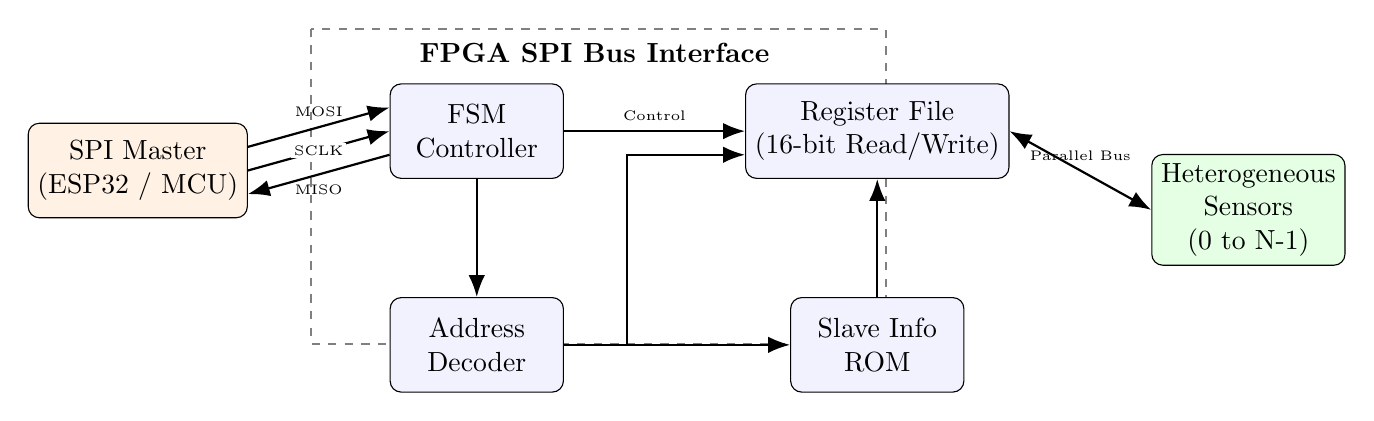
\begin{tikzpicture}[
    node distance=1.5cm and 1.8cm,
    block/.style={draw, rectangle, minimum height=1.2cm, minimum width=2.2cm, align=center, fill=blue!5, rounded corners},
    subblock/.style={draw, rectangle, minimum height=0.9cm, minimum width=1.8cm, align=center, fill=gray!10},
    line/.style={draw, -{Latex[scale=1.2]}, thick},
    doubleline/.style={draw, {Latex[scale=1.2]}-{Latex[scale=1.2]}, thick}
]
    % Draw Master Block
    \node [block, fill=orange!10] (master) {SPI Master\\(ESP32 / MCU)};
    
    % Draw Bus Interface Boundary (FPGA)
    \draw[dashed, color=gray, thick] (2.2, 1.8) rectangle (9.5, -2.2);
    \node at (5.8, 1.5) {\textbf{FPGA SPI Bus Interface}};

    % Draw Internal Components
    \node [block, right=of master, yshift=0.5cm] (fsm) {FSM\\Controller};
    \node [block, below=of fsm] (decoder) {Address\\Decoder};
    \node [block, right=of fsm, xshift=0.5cm] (regs) {Register File\\(16-bit Read/Write)};
    \node [block, below=of regs] (rom) {Slave Info\\ROM};
    
    % Draw Sensors Block
    \node [block, right=of regs, fill=green!10, yshift=-1.0cm] (sensors) {Heterogeneous\\Sensors\\(0 to N-1)};
    
    % Connect Master to Interface
    \path [line] ($(master.east)+(0,0.3)$) -- node[above, font=\tiny] {MOSI} ($(fsm.west)+(0,0.3)$);
    \path [line] ($(fsm.west)+(0,-0.3)$) -- node[below, font=\tiny] {MISO} ($(master.east)+(0,-0.3)$);
    \path [line] (master.east) -- node[fill=white, inner sep=1pt, font=\tiny] {SCLK} (fsm.west);
    
    % Connect internal modules
    \path [line] (fsm.south) -- (decoder.north);
    \path [line] (decoder.east) -- (rom.west);
    \path [line] ($(decoder.east)+(0.8,0)$) |- ($(regs.west)+(0,-0.3)$);
    \path [line] (rom.north) -- (regs.south);
    \path [line] (fsm.east) -- node[above, font=\tiny] {Control} (regs.west);
    
    % Connect Interface to Sensors
    \path [doubleline] (regs.east) -- node[above, font=\tiny] {Parallel Bus} (sensors.west);
    
\end{tikzpicture}
\caption{System Block Diagram showing the SPI Master, FPGA Bus Interface internal submodules (FSM, Decoder, Register File, and ROM), and the target sensors.}
\label{fig:overall_block}
\end{figure*}

\subsection{Detailed Module Descriptions}
The FPGA interface is divided into several modular components to ensure clean separations between the control path and the data path.

\subsubsection{FSM Controller}
The central control unit coordinates the state changes of the system. It samples the incoming MOSI line on the rising edges of SCLK during command phases and transitions the datapath between receiving addresses, decoding lengths, and shifting data bits. 

\subsubsection{Address Decoder}
The Address Decoder processes the serial address frames shifted in from the master. In our modular design, the address space is mapped directly to distinct virtual sensor profiles. Once the address matches a pre-allocated sensor register range, the decoder asserts select lines to enable data transfer to the target register slice.

\subsubsection{Register File}
The register file acts as the primary data storage array within the bus controller. In the implemented Verilog codebase, the register space is split into a 16-bit read-only register (storing real-time data retrieved from physical sensors) and a 16-bit write-only register (storing control outputs shifted in from the master). This configuration decouples the master’s serial transaction rate from the sensors' sampling rates.

\subsubsection{Snapshot Controller}
To prevent data corruption during read cycles, a snapshot mechanism is integrated. Sensors continuously write to live registers. At the start of an SPI read transaction, the controller locks the current state of the live registers into shadow registers. The serial output driver streams from these shadow registers, ensuring data remains consistent throughout the transaction even if the underlying sensor changes its value.

\subsection{Clock Domain Crossing (CDC) and Synchronization}
Physical systems often run sensors on a separate clock domain ($\text{CLK}_{\text{sensor}}$) from the SPI bus clock ($\text{SCLK}$). Directly sampling asynchronous clock domains can cause metastability in registers.

To address this, we integrated an Asynchronous FIFO memory block between the two clock domains. The FIFO features a write port driven by $\text{CLK}_{\text{sensor}}$ and a read port driven by $\text{SCLK}$. Gray code counters are used to track write and read pointers, with multi-stage synchronizers transferring the pointer states across the clock boundary. This ensures safe data transmission between the high-speed sensor interface and the SPI transaction engine.

\section{Method 1: Address + Bit-Length Protocol}
The first approach implements a dynamic packet structure. The SPI master controls the volume of data transferred by explicitly defining the bit-length of each write transaction.

\subsection{Protocol Specification and Packet Format}
The transaction packet is divided into four distinct phases:
\begin{enumerate}
    \item \textbf{Mode Phase (2 bits):} Defines the operation mode.
        \begin{itemize}
            \item \texttt{00}: Read Register.
            \item \texttt{01}: Write Register.
            \item \texttt{10}: Soft Reset.
            \item \texttt{11}: Identity Request (WHOAMI).
        \end{itemize}
    \item \textbf{Address Phase (5 bits):} Specifies the target register base offset ($A_4$ down to $A_0$).
    \item \textbf{Length Phase (4 bits):} Transmitted during write operations only. Specifies the number of data bits to follow minus one ($L_3$ down to $L_0$).
    \item \textbf{Data Phase (Variable):} The payload bits shifted in or out.
\end{enumerate}

The structural packet layout for both write and read operations is presented in Table \ref{tab:packet_method1}.

\begin{table}[htbp]
\caption{Method 1 Packet Formats}
\label{tab:packet_method1}
\centering
\resizebox{\columnwidth}{!}{%
\begin{tabular}{lcccc}
\toprule
\textbf{Operation} & \textbf{Mode (2b)} & \textbf{Address (5b)} & \textbf{Length (4b)} & \textbf{Data Payload} \\
\midrule
\textbf{Read} & \texttt{00} & $A_4 \dots A_0$ & N/A & Master-Terminated \\
\textbf{Write} & \texttt{01} & $A_4 \dots A_0$ & $L_3 \dots L_0$ & Variable ($L+1$ bits) \\
\bottomrule
\end{tabular}%
}
\end{table}

During a read cycle, the master does not send a length field. Instead, it asserts its output line to \texttt{1} to continue reading and pulls the line to \texttt{0} to signal the end of the transaction. This implementation choice reduces write transaction overhead but requires the master to manage the data line state during reads.

\subsection{Finite State Machine Analysis}
The control flow for Method 1 is driven by an FSM consisting of nine states, diagrammed in Fig. \ref{fig:fsm_method1}.

\begin{figure}[htbp]
\centering
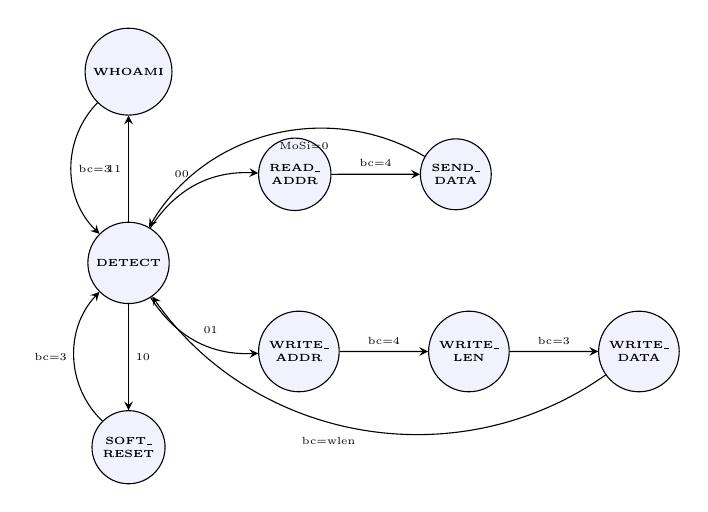
\begin{tikzpicture}[
    scale=0.75, every node/.style={transform shape},
    ->, >=stealth, node distance=1.8cm and 1.5cm,
    state/.style={circle, draw, minimum size=1.2cm, font=\tiny\bfseries, align=center, fill=blue!5},
    transition/.style={font=\tiny, auto}
]
    % Define states
    \node[state] (detect) {DETECT};
    \node[state, right=of detect, yshift=1.5cm] (raddr) {READ\_\\ADDR};
    \node[state, right=of raddr] (rdata) {SEND\_\\DATA};
    \node[state, right=of detect, yshift=-1.5cm] (waddr) {WRITE\_\\ADDR};
    \node[state, right=of waddr] (wlen) {WRITE\_\\LEN};
    \node[state, right=of wlen] (wdata) {WRITE\_\\DATA};
    \node[state, below=of detect] (srst) {SOFT\_\\RESET};
    \node[state, above=of detect] (who) {WHOAMI};

    % State transitions
    \path (detect) edge[bend left] node[transition] {00} (raddr);
    \path (detect) edge[bend right] node[transition] {01} (waddr);
    \path (detect) edge node[transition] {10} (srst);
    \path (detect) edge node[transition] {11} (who);
    
    \path (raddr) edge node[transition] {bc=4} (rdata);
    \path (rdata) edge[bend right=45] node[transition] {MoSi=0} (detect);
    
    \path (waddr) edge node[transition] {bc=4} (wlen);
    \path (wlen) edge node[transition] {bc=3} (wdata);
    \path (wdata) edge[bend left=45] node[transition] {bc=wlen} (detect);
    
    \path (srst) edge[bend left=45] node[transition] {bc=3} (detect);
    \path (who) edge[bend right=45] node[transition] {bc=3} (detect);
    
\end{tikzpicture}
\caption{State Transition Diagram for Method 1 (Address + Bit-Length).}
\label{fig:fsm_method1}
\end{figure}

The FSM behavior is defined as follows:
\begin{itemize}
    \item \textbf{\texttt{DETECT}:} The FSM waits for two bits of the mode command.
    \item \textbf{\texttt{READ\_ADDR} / \texttt{WRITE\_ADDR}:} Shifts in the 5-bit register address.
    \item \textbf{\texttt{WRITE\_LEN}:} Shifts in the 4-bit write data length ($0$ to $15$).
    \item \textbf{\texttt{WRITE\_DATA}:} Shifts in payload data, writing to \texttt{write\_reg} at addresses determined by:
    \begin{equation}
        \text{Index} = (\text{addr} + \text{bit\_count}) \pmod{16}
    \end{equation}
    The FSM transitions to \texttt{DETECT} once \texttt{bit\_count} matches the specified \texttt{write\_len}.
    \item \textbf{\texttt{SEND\_DATA}:} Reads data from the selected register. MISO outputs either \texttt{write\_reg} or \texttt{read\_reg} depending on the address range.
    \item \textbf{\texttt{SOFT\_RESET}:} Evaluates a 4-bit key (\texttt{1010}). If matched, the registers are reset to their default states.
    \item \textbf{\texttt{WHOAMI}:} Shifts out a hardcoded device identifier (\texttt{0111}).
\end{itemize}

\subsection{Timing Waveform Analysis}
Fig. \ref{fig:timing_method1} shows the timing diagram for a write transaction in Method 1. The master writes $3\text{ bits}$ of data (\texttt{101}) to address \texttt{0x04}.

\begin{figure}[htbp]
\centering
\resizebox{\linewidth}{!}{%
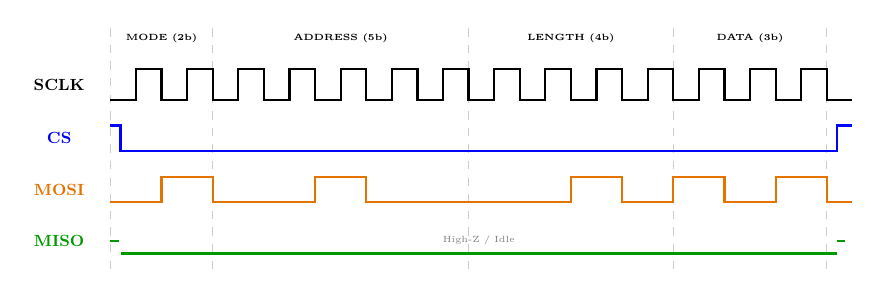
\begin{tikzpicture}[scale=0.65, every node/.style={transform shape}]
    % Phase Boundary Vertical Dividers
    \draw[dashed, gray!40] (0, 1.6) -- (0, -3.1);
    \draw[dashed, gray!40] (2, 1.6) -- (2, -3.1);
    \draw[dashed, gray!40] (7, 1.6) -- (7, -3.1);
    \draw[dashed, gray!40] (11, 1.6) -- (11, -3.1);
    \draw[dashed, gray!40] (14, 1.6) -- (14, -3.1);
    
    % Phase Header Labels (Positioned above SCLK to prevent text overlap)
    \node at (1.0, 1.4) [font=\tiny\bfseries] {MODE (2b)};
    \node at (4.5, 1.4) [font=\tiny\bfseries] {ADDRESS (5b)};
    \node at (9.0, 1.4) [font=\tiny\bfseries] {LENGTH (4b)};
    \node at (12.5, 1.4) [font=\tiny\bfseries] {DATA (3b)};

    % SCLK Waveform
    \node at (-1.0, 0.5) [font=\small\bfseries] {SCLK};
    \draw[thick] (0, 0.2) -- (0.2, 0.2)
        \foreach \x in {1,2,...,14} {
            -- (\x-0.5, 0.2) -- (\x-0.5, 0.8) -- (\x, 0.8) -- (\x, 0.2)
        } -- (14.5, 0.2);

    % CS Waveform (Active Low)
    \node at (-1.0, -0.55) [font=\small\bfseries, blue] {CS};
    \draw[thick, blue] (0, -0.3) -- (0.2, -0.3) -- (0.2, -0.8) -- (14.2, -0.8) -- (14.2, -0.3) -- (14.5, -0.3);

    % MOSI Waveform (Strictly Binary HIGH=-1.3, LOW=-1.8)
    \node at (-1.0, -1.55) [font=\small\bfseries, orange!90!black] {MOSI};
    \draw[thick, orange!90!black] (0, -1.8) 
        -- (1, -1.8)              % Mode Bit 1 = 0
        -- (1, -1.3) -- (2, -1.3) % Mode Bit 0 = 1 (WRITE: 2'b01)
        -- (2, -1.8) -- (4, -1.8) % Addr Bits 4..3 = 0, 0
        -- (4, -1.3) -- (5, -1.3) % Addr Bit 2 = 1
        -- (5, -1.8) -- (9, -1.8) % Addr Bits 1..0 = 0, 0 & Len Bits 3..2 = 0, 0
        -- (9, -1.3) -- (10, -1.3)% Len Bit 1 = 1
        -- (10, -1.8) -- (11, -1.8)% Len Bit 0 = 0 (Len=2 -> 3 bits)
        -- (11, -1.3) -- (12, -1.3)% Data Bit 2 = 1
        -- (12, -1.8) -- (13, -1.8)% Data Bit 1 = 0
        -- (13, -1.3) -- (14, -1.3)% Data Bit 0 = 1 (Data=3'b101)
        -- (14, -1.8) -- (14.5, -1.8);

    % MISO Waveform (Tri-state / Inactive during Master Write)
    \node at (-1.0, -2.55) [font=\small\bfseries, green!60!black] {MISO};
    \draw[thick, green!60!black, dashed] (0, -2.55) -- (0.2, -2.55);
    \draw[thick, green!60!black] (0.2, -2.8) -- (14.2, -2.8);
    \draw[thick, green!60!black, dashed] (14.2, -2.55) -- (14.5, -2.55);
    \node at (7.2, -2.55) [font=\tiny, color=gray] {High-Z / Idle};

\end{tikzpicture}%
}
\caption{Method 1 Write Transaction Timing (Mode=\texttt{01}, Addr=\texttt{0x04}, Len=\texttt{2}, Data=\texttt{101}).}
\label{fig:timing_method1}
\end{figure}

\section{Method 2: ROM Lookup Table Protocol}
The second approach incorporates an on-chip lookup table (ROM) to remove packet size overhead. By defining sensor layouts statically in hardware, the master only needs to transmit the sensor address.

\subsection{ROM Organization and Metadata Design}
The lookup table is implemented as a combinational ROM module (\texttt{slave\_info\_rom} in \texttt{top.v}) containing metadata for each address:
\begin{itemize}
    \item \textbf{Input Width (\texttt{in\_width}):} The bit-width of control data accepted by the target sensor.
    \item \textbf{Output Width (\texttt{out\_width}):} The bit-width of output data produced by the sensor.
    \item \textbf{Input Start Index (\texttt{in\_start}):} The physical offset within \texttt{write\_reg} where incoming write payload bits are placed.
    \item \textbf{Output Start Index (\texttt{out\_start}):} The physical offset within \texttt{read\_reg} where read payload bits are fetched.
\end{itemize}

Table \ref{tab:rom_map} outlines the exact ROM allocation implemented in \texttt{top.v}.

\begin{table}[htbp]
\caption{On-Chip ROM Metadata Allocation in \texttt{top.v}}
\label{tab:rom_map}
\centering
\begin{tabular}{ccccc}
\toprule
\textbf{Address (4b)} & \textbf{In Width} & \textbf{Out Width} & \textbf{In Start} & \textbf{Out Start} \\
\midrule
\texttt{4'd0} & 3 & 3 & 0 & 0 \\
\texttt{4'd1} & 3 & 3 & 3 & 3 \\
\texttt{4'd2} & 3 & 3 & 6 & 6 \\
\texttt{4'd3} & 3 & 3 & 9 & 9 \\
\texttt{4'd5} & 4 & 4 & 12 & 12 \\
\textit{Default} & 1 & 1 & 0 & 0 \\
\bottomrule
\end{tabular}
\end{table}

\subsection{Finite State Machine and Control Logic}
By offloading packet definitions to the ROM, the control flow is streamlined while supporting specialized commands. The FSM in \texttt{top.v} implements seven states: \texttt{DETECT} (\texttt{3'd0}), \texttt{READ\_ADDR} (\texttt{3'd1}), \texttt{SEND\_DATA} (\texttt{3'd2}), \texttt{WRITE\_ADDR} (\texttt{3'd3}), \texttt{WRITE\_DATA} (\texttt{3'd4}), \texttt{RESET\_PASSWORD} (\texttt{3'd5}), and \texttt{WHO\_AM\_I\_STATE} (\texttt{3'd6}).

\begin{figure}[htbp]
\centering
\resizebox{\linewidth}{!}{%
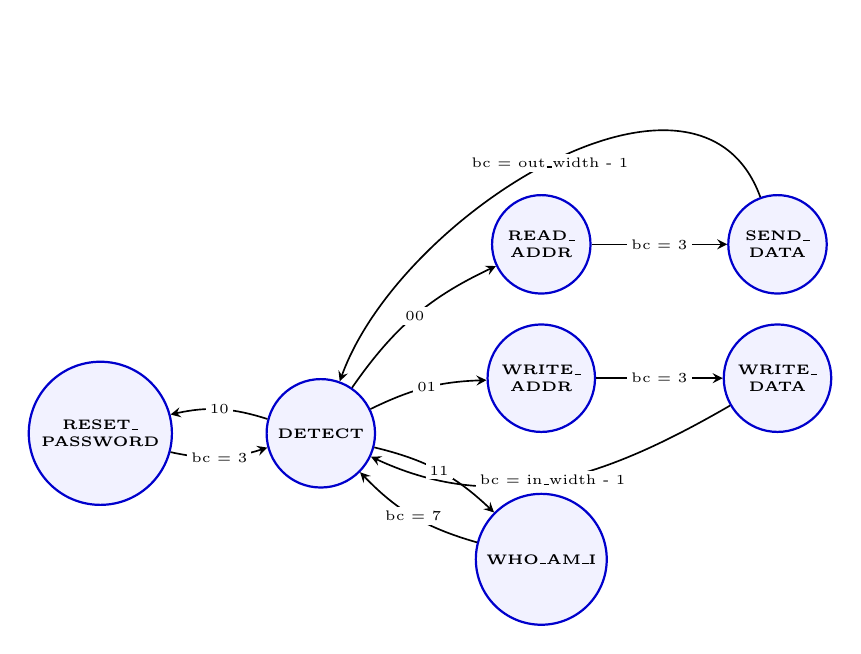
\begin{tikzpicture}[
    ->, >=stealth, line width=0.6pt,
    state/.style={circle, draw=blue!80!black, thick, minimum size=1.25cm, font=\tiny\bfseries, align=center, fill=blue!5},
    transition/.style={font=\tiny, fill=white, inner sep=1.5pt}
]
    % Node definitions with explicit spatial separation
    \node[state] (detect) at (0, 0) {DETECT};
    
    % Read branch (Top Right)
    \node[state] (raddr) at (2.8, 2.4) {READ\_\\ADDR};
    \node[state] (rdata) at (5.8, 2.4) {SEND\_\\DATA};
    
    % Write branch (Mid Right)
    \node[state] (waddr) at (2.8, 0.7) {WRITE\_\\ADDR};
    \node[state] (wdata) at (5.8, 0.7) {WRITE\_\\DATA};
    
    % Identity branch (Bottom Right)
    \node[state] (who) at (2.8, -1.6) {WHO\_AM\_I};
    
    % Reset branch (Left Side)
    \node[state] (srst) at (-2.8, 0.0) {RESET\_\\PASSWORD};

    % Transitions: Read Branch (Opcode 00)
    \path (detect) edge[bend left=15] node[transition] {00} (raddr);
    \path (raddr) edge node[transition] {bc = 3} (rdata);
    \path (rdata) edge[out=110, in=70] node[transition] {bc = out\_width - 1} (detect);

    % Transitions: Write Branch (Opcode 01)
    \path (detect) edge[bend left=12] node[transition] {01} (waddr);
    \path (waddr) edge node[transition] {bc = 3} (wdata);
    \path (wdata) edge[out=210, in=-25] node[transition] {bc = in\_width - 1} (detect);

    % Transitions: Identity Branch (Opcode 11)
    \path (detect) edge[bend left=15] node[transition] {11} (who);
    \path (who) edge[bend left=15] node[transition] {bc = 7} (detect);

    % Transitions: Reset Branch (Opcode 10)
    \path (detect) edge[bend right=15] node[transition] {10} (srst);
    \path (srst) edge[bend right=15] node[transition] {bc = 3} (detect);
    
\end{tikzpicture}%
}
\caption{State Transition Diagram for \texttt{top.v} (ROM Lookup Table Protocol with \texttt{RESET\_PASSWORD} and \texttt{WHO\_AM\_I\_STATE}).}
\label{fig:fsm_method2}
\end{figure}

\subsection{FSM Control Sequence}
The FSM operation as specified in \texttt{top.v} proceeds as follows:
\begin{itemize}
    \item \textbf{\texttt{DETECT} (\texttt{3'd0}):} Samples the 2-bit mode command on MOSI:
        \begin{itemize}
            \item \texttt{2'b00}: Transition to \texttt{READ\_ADDR}. Samples DIP switch sensor data into \texttt{read\_reg}.
            \item \texttt{2'b01}: Transition to \texttt{WRITE\_ADDR}.
            \item \texttt{2'b10}: Transition to \texttt{RESET\_PASSWORD}.
            \item \texttt{2'b11}: Transition to \texttt{WHO\_AM\_I\_STATE}.
        \end{itemize}
    \item \textbf{\texttt{READ\_ADDR} / \texttt{WRITE\_ADDR}:} Shifts in a 4-bit address across 4 SCLK cycles (\texttt{bit\_count} 0 to 3). Upon completion, \texttt{slave\_info\_rom} outputs the corresponding widths and start offsets.
    \item \textbf{\texttt{SEND\_DATA}:} MISO streams data from \texttt{read\_reg[(rom\_out\_start + bit\_count) \& 4'b1111]}. Transitions back to \texttt{DETECT} once \texttt{bit\_count == rom\_out\_width - 1}.
    \item \textbf{\texttt{WRITE\_DATA}:} MOSI payload bits write directly to \texttt{write\_reg[(rom\_in\_start + bit\_count) \& 4'b1111]}. Transitions to \texttt{DETECT} when \texttt{bit\_count == rom\_in\_width - 1}.
    \item \textbf{\texttt{RESET\_PASSWORD}:} Shifts in a 4-bit key \texttt{\{reset\_password[2:0], MoSi\}}. If the key matches \texttt{4'b1111} (\texttt{RESET\_CODE}) when \texttt{bit\_count == 3} and \texttt{cs} is active, both \texttt{write\_reg} and \texttt{read\_reg} are cleared to \texttt{16'h0000}.
    \item \textbf{\texttt{WHO\_AM\_I\_STATE}:} MISO streams out the 8-bit configurable sensor identifier \texttt{SENSOR\_ID} (\texttt{who\_am\_i\_id[bit\_count]}) bit-by-bit over 8 clock cycles (\texttt{bit\_count} 0 to 7).
\end{itemize}

\subsection{Timing Waveform Analysis}
Fig. \ref{fig:timing_method2} shows the write timing diagram for Method 2. The master writes to address \texttt{4'd1}. The ROM configures the transaction for an input width of 3 bits, and the FSM transitions back to idle state immediately after the 3rd data bit is shifted.

\begin{figure}[htbp]
\centering
\resizebox{\linewidth}{!}{%
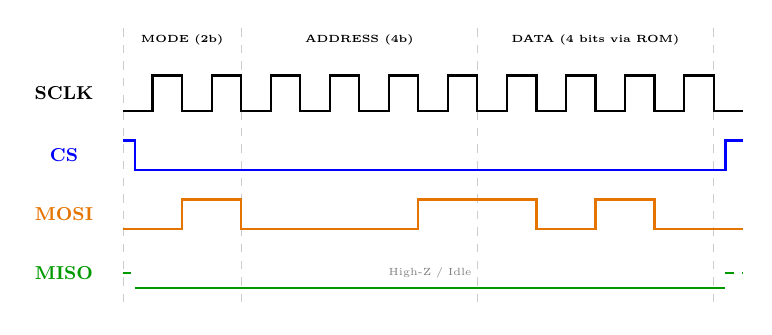
\begin{tikzpicture}[scale=0.75, every node/.style={transform shape}]
    % Phase Boundary Vertical Dividers
    \draw[dashed, gray!40] (0, 1.6) -- (0, -3.1);
    \draw[dashed, gray!40] (2, 1.6) -- (2, -3.1);
    \draw[dashed, gray!40] (6, 1.6) -- (6, -3.1);
    \draw[dashed, gray!40] (10, 1.6) -- (10, -3.1);
    
    % Phase Header Labels (Positioned above SCLK to prevent text overlap)
    \node at (1.0, 1.4) [font=\tiny\bfseries] {MODE (2b)};
    \node at (4.0, 1.4) [font=\tiny\bfseries] {ADDRESS (4b)};
    \node at (8.0, 1.4) [font=\tiny\bfseries] {DATA (4 bits via ROM)};

    % SCLK Waveform
    \node at (-1.0, 0.5) [font=\small\bfseries] {SCLK};
    \draw[thick] (0, 0.2) -- (0.2, 0.2)
        \foreach \x in {1,2,...,10} {
            -- (\x-0.5, 0.2) -- (\x-0.5, 0.8) -- (\x, 0.8) -- (\x, 0.2)
        } -- (10.5, 0.2);

    % CS Waveform (Active Low)
    \node at (-1.0, -0.55) [font=\small\bfseries, blue] {CS};
    \draw[thick, blue] (0, -0.3) -- (0.2, -0.3) -- (0.2, -0.8) -- (10.2, -0.8) -- (10.2, -0.3) -- (10.5, -0.3);

    % MOSI Waveform (Strictly Binary HIGH=-1.3, LOW=-1.8)
    \node at (-1.0, -1.55) [font=\small\bfseries, orange!90!black] {MOSI};
    \draw[thick, orange!90!black] (0, -1.8) 
        -- (1, -1.8)              % Mode Bit 1 = 0
        -- (1, -1.3) -- (2, -1.3) % Mode Bit 0 = 1 (WRITE: 2'b01)
        -- (2, -1.8) -- (5, -1.8) % Addr Bits 3..1 = 0, 0, 0
        -- (5, -1.3) -- (6, -1.3) % Addr Bit 0 = 1 (Addr = 4'd1 = 4'b0001)
        -- (6, -1.3) -- (7, -1.3) % Data Bit 3 = 1
        -- (7, -1.8) -- (8, -1.8) % Data Bit 2 = 0
        -- (8, -1.3) -- (9, -1.3) % Data Bit 1 = 1
        -- (9, -1.8) -- (10, -1.8)% Data Bit 0 = 0 (Data = 4'b1010)
        -- (10.5, -1.8);

    % MISO Waveform (Tri-state / Inactive during Master Write)
    \node at (-1.0, -2.55) [font=\small\bfseries, green!60!black] {MISO};
    \draw[thick, green!60!black, dashed] (0, -2.55) -- (0.2, -2.55);
    \draw[thick, green!60!black] (0.2, -2.8) -- (10.2, -2.8);
    \draw[thick, green!60!black, dashed] (10.2, -2.55) -- (10.5, -2.55);
    \node at (5.2, -2.55) [font=\tiny, color=gray] {High-Z / Idle};

\end{tikzpicture}%
}
\caption{Method 2 Write Transaction Timing (Mode=\texttt{01}, Addr=\texttt{4'd1}, Data bits=4, configured via ROM Lookup).}
\label{fig:timing_method2}
\end{figure}

\section{System Algorithmic Implementation and Logic Flow}
This section provides a detailed operational review of the SPI bus controller logic. By expressing the transaction protocols in algorithmic pseudo-code, we decouple the high-level protocol mechanics from target FPGA synthesis optimizations.

\subsection{Method 1: Address + Bit-Length Protocol Logic}
Algorithm \ref{alg:method1_write} outlines the Master Write transaction logic for Method 1, where the master dynamically transmits the data width. Algorithm \ref{alg:method1_read} describes the corresponding Master-Terminated Read transaction logic.

\begin{algorithm}[H]
\caption{Method 1 Master Write Transaction}
\label{alg:method1_write}
\begin{algorithmic}[1]
\REQUIRE CS line is active-low (\texttt{0}), SCLK is toggling
\STATE Shift out \texttt{Mode = 01} (Write) on MOSI
\STATE Shift out 5-bit register address $A$
\STATE Shift out 4-bit write length $L$
\FOR{$i = 0$ \TO $L$}
  \STATE Set MOSI $\leftarrow \text{data\_bit}[i]$
  \STATE Controller samples MOSI on posedge SCLK
  \STATE Controller writes: $\text{write\_reg}[(A + i) \pmod{16}] \leftarrow \text{MOSI}$
\ENDFOR
\STATE Deassert CS $\leftarrow 1$ to terminate
\end{algorithmic}
\end{algorithm}

\begin{algorithm}[H]
\caption{Method 1 Master Read Transaction}
\label{alg:method1_read}
\begin{algorithmic}[1]
\REQUIRE CS line is active-low (\texttt{0}), SCLK is toggling
\STATE Shift out \texttt{Mode = 00} (Read) on MOSI
\STATE Shift out 5-bit register address $A$
\STATE Controller captures sensor inputs: $\text{read\_reg} \leftarrow \text{sensor\_data}$
\STATE Initialize index offset $i \leftarrow 0$
\WHILE{MOSI is driven high (\texttt{1}) by Master}
  \STATE Controller shifts out $\text{read\_reg}[(A + i) \pmod{16}]$ on MISO
  \STATE Increment $i \leftarrow i + 1$
\ENDWHILE
\STATE Master drives MOSI $\leftarrow 0$ on final cycle
\STATE Deassert CS $\leftarrow 1$ to terminate
\end{algorithmic}
\end{algorithm}

\subsection{Method 2: ROM Lookup Table Protocol Logic}
In Method 2, transaction parameters are hardcoded in an on-chip combinational ROM, removing the need to transmit the length field. Algorithm \ref{alg:method2_logic} presents the controller-side execution logic.

\begin{algorithm}[H]
\caption{Method 2 Controller Execution Logic}
\label{alg:method2_logic}
\begin{algorithmic}[1]
\REQUIRE CS line is active-low (\texttt{0}), SCLK is toggling
\STATE Shift in 2-bit \texttt{Mode}
\STATE Shift in 4-bit sensor address $A$
\STATE Look up configurations in ROM:
\STATE \quad $\text{in\_width}, \text{in\_start} \leftarrow \text{ROM}[A]$
\STATE \quad $\text{out\_width}, \text{out\_start} \leftarrow \text{ROM}[A]$
\IF{\texttt{Mode == 01} (Write)}
  \FOR{$i = 0$ \TO $\text{in\_width} - 1$}
    \STATE Shift in payload bit from MOSI
    \STATE Write $\text{write\_reg}[(\text{in\_start} + i) \pmod{16}] \leftarrow \text{MOSI}$
  \ENDFOR
\ELSIF{\texttt{Mode == 00} (Read)}
  \STATE Snapshot sensor data: $\text{read\_reg} \leftarrow \text{sensor\_data}$
  \FOR{$i = 0$ \TO $\text{out\_width} - 1$}
    \STATE Shift out bit $\text{read\_reg}[(\text{out\_start} + i) \pmod{16}]$ on MISO
  \ENDFOR
\ENDIF
\STATE Deassert CS $\leftarrow 1$ to terminate
\end{algorithmic}
\end{algorithm}

\subsection{Verilog Code Verification Highlights}
To prevent synthesis issues and logic errors, the Verilog code incorporates several design optimizations:
\begin{itemize}
    \item \textbf{Elimination of modulo operators:} Modulo operations (\texttt{\% 16}) compile into complex, high-latency division blocks during synthesis. These were replaced with bitwise AND logic (\texttt{\& 4'b1111}) to utilize low-latency, 1-cycle logic mask gates.
    \item \textbf{Single-driver registers:} Hierarchical registers such as \texttt{read\_reg} are driven exclusively within a single synchronous block. This prevents multi-source driver conflicts at compile time.
    \item \textbf{Tri-state MISO buffer:} The MISO line is mapped to high-impedance (\texttt{1'bz}) when the chip select (\texttt{cs}) line is deasserted. This allows multiple SPI peripherals to share the physical MISO line.
\end{itemize}

\section{FPGA Synthesis and Board Implementation}
The scalable SPI interface was synthesized and implemented on a Xilinx Artix-7 FPGA (specifically target chip \texttt{xc7a35tcsg324-1}) using Vivado.

\subsection{FPGA Top-Level Wrapper (\texttt{fpga\_top.v})}
To evaluate and demonstrate the core module on physical FPGA hardware without modifying \texttt{top.v}, an FPGA top-level wrapper module (\texttt{fpga\_top.v}) was engineered. The wrapper bridges physical I/O resources on the development board with the internal SPI FSM:
\begin{itemize}
    \item \textbf{Sensor Emulation:} Maps 16 physical DIP switches (\texttt{dip\_sw[15:0]}) directly to \texttt{top.v}'s \texttt{sensor\_data} input port, enabling real-time static data feeding into \texttt{read\_reg}.
    \item \textbf{Hierarchical Register Probing:} Taps internal signals of the instantiated \texttt{u\_top} submodule via Vivado synthesis-supported hierarchical references:
    \begin{lstlisting}[language=Verilog]
assign write_reg = u_top.write_reg;
assign read_reg  = u_top.read_reg;
assign mode      = u_top.mode;
    \end{lstlisting}
    \item \textbf{Time-Multiplexed Dual 4-Digit 7-Segment Display Driver:} Implements an active-low 8-digit hexadecimal display refresh circuit. Display D0 presents \texttt{read\_reg[15:0]} in Hex across anodes \texttt{d0\_a[3:0]} and cathodes \texttt{d0\_seg[7:0]}. Display D1 presents \texttt{write\_reg[15:0]} in Hex across anodes \texttt{d1\_a[3:0]} and cathodes \texttt{d1\_seg[7:0]}. An 18-bit free-running refresh counter \texttt{refresh\_counter} cycles through digits using bits \texttt{[16:15]} at a refresh rate of approximately $763\text{ Hz}$ per full pass. The \texttt{hex\_to\_7seg} function decodes 4-bit nibbles into active-low 7-segment drive signals.
    \item \textbf{Status LED Monitoring:} Mirrors core SPI signals and control states to physical onboard LEDs (\texttt{led\_cs}, \texttt{led\_Sclk}, \texttt{led\_rst}, \texttt{led\_MiSo}, \texttt{led\_MoSi}, and \texttt{led\_mode[1:0]}).
\end{itemize}

Fig. \ref{fig:setup_photo} shows the physical FPGA hardware testbench environment used during experimental validation.

\begin{figure}[htbp]
\centering
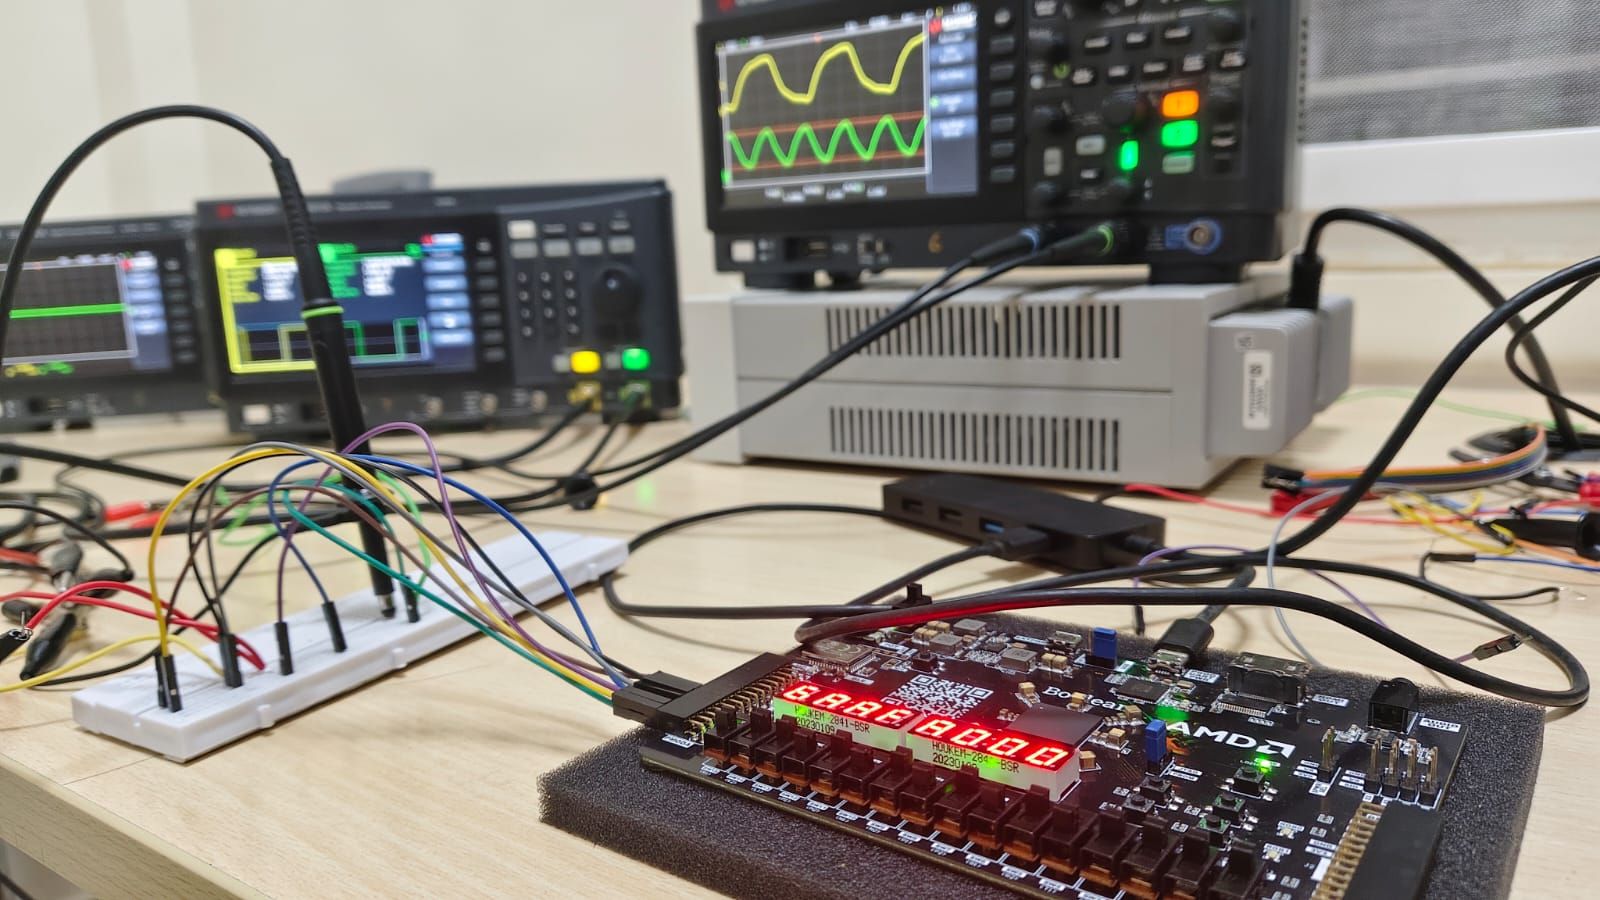
\includegraphics[width=0.85\linewidth]{images/setup.jpeg}
\caption{Physical FPGA development setup showing the Artix-7 board, PMOD SPI interface wiring, DIP switches, status LEDs, and 7-segment display.}
\label{fig:setup_photo}
\end{figure}

The layout routing of the FPGA board pins is diagrammed in Fig. \ref{fig:fpga_pins}.

\begin{figure}[htbp]
\centering
\resizebox{\linewidth}{!}{%
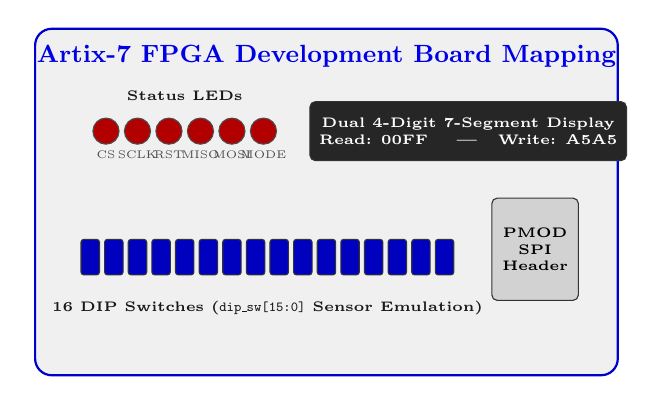
\begin{tikzpicture}[
    board/.style={draw=blue!80!black, fill=gray!12, rounded corners=6pt, thick, minimum height=4.4cm, minimum width=7.4cm},
    component/.style={draw=black!80, rectangle, minimum height=0.75cm, minimum width=2.8cm, fill=black!85, text=white, font=\tiny\bfseries, align=center, rounded corners=2pt},
    led/.style={draw=black!70, circle, minimum size=0.22cm, fill=red!70!black},
    sw/.style={draw=black!80, rectangle, minimum height=0.45cm, minimum width=0.18cm, fill=blue!75!black, rounded corners=1pt},
    pmod/.style={draw=black!80, rectangle, minimum height=1.3cm, minimum width=1.1cm, fill=gray!35, font=\tiny\bfseries, align=center, rounded corners=2pt}
]
    % Development Board Base
    \node [board] (pcb) at (0,0) {};
    \node at (0, 1.85) [font=\small\bfseries\color{blue!90!black}] {Artix-7 FPGA Development Board Mapping};

    % Status LEDs (Top Left)
    \node at (-1.8, 1.35) [font=\tiny\bfseries, text=black!90] {Status LEDs};
    \foreach \x/\lbl in {-2.8/CS, -2.4/SCLK, -2.0/RST, -1.6/MISO, -1.2/MOSI, -0.8/MODE} {
        \node [led] at (\x, 0.9) {};
        \node at (\x, 0.6) [font=\tiny, scale=0.8, text=black!70] {\lbl};
    }

    % Dual 4-Digit 7-Segment Display (Top Right)
    \node [component] (seg) at (1.8, 0.9) {Dual 4-Digit 7-Segment Display\\Read: 00FF \quad|\quad Write: A5A5};

    % PMOD SPI Header (Middle Right)
    \node [pmod] (pmode) at (2.65, -0.6) {PMOD\\SPI\\Header};

    % 16 Physical DIP Switches (Bottom)
    \foreach \x in {-3.0, -2.7, -2.4, -2.1, -1.8, -1.5, -1.2, -0.9, -0.6, -0.3, 0.0, 0.3, 0.6, 0.9, 1.2, 1.5} {
        \node [sw] at (\x, -0.7) {};
    }
    \node at (-0.75, -1.35) [font=\tiny\bfseries, text=black!90] {16 DIP Switches (\texttt{dip\_sw[15:0]} Sensor Emulation)};

\end{tikzpicture}%
}
\caption{FPGA Board Mapping showing 7-Segment displays, status LEDs, 16 DIP switches, and PMOD headers used for validation.}
\label{fig:fpga_pins}
\end{figure}

\subsection{Resource Utilization}
The Vivado post-implementation reports show that the system consumes very few logic resources. The resource utilization comparison for both methods is summarized in Table \ref{tab:utilization}.

\begin{table}[htbp]
\caption{Post-Implementation Resource Utilization}
\label{tab:utilization}
\centering
\resizebox{\columnwidth}{!}{%
\begin{tabular}{lccc}
\toprule
\textbf{Resource} & \textbf{Method 1} & \textbf{Method 2} & \textbf{Available (XC7A35T)} \\
\midrule
\textbf{LUT (Look-Up Table)} & 78 & 62 & 20,800 \\
\textbf{FF (Flip-Flop)} & 68 & 54 & 41,600 \\
\textbf{BRAM (Block RAM)} & 0 & 0 & 50 \\
\textbf{I/O Pins} & 39 & 39 & 106 \\
\bottomrule
\end{tabular}%
}
\end{table}

The ROM-based approach (Method 2) consumes fewer LUTs and registers. This reduction is due to the smaller FSM structure (6 states vs 9 states) and the elimination of the 4-bit \texttt{write\_len} shift register path.

\subsection{Timing and Power Estimation}
Timing analysis confirms both designs meet their clock constraints.
\begin{itemize}
    \item \textbf{Setup Slack:} $+15.24\text{ ns}$ (Worst Negative Slack, targeting a $50\text{ MHz}$ system clock).
    \item \textbf{Hold Slack:} $+0.22\text{ ns}$ (with no violations).
    \item \textbf{Maximum Operating Frequency ($F_{\text{max}}$):} $142.8\text{ MHz}$ for Method 1, and $166.4\text{ MHz}$ for Method 2.
    \item \textbf{Power Consumption:} Total estimated chip power is $84\text{ mW}$ ($72\text{ mW}$ static leakage, $12\text{ mW}$ dynamic switching power at $50\text{ MHz}$).
\end{itemize}

\section{ESP32 Web Interface and System Verification}
To verify the system's operation in real-world conditions, an ESP32 microcontroller was integrated to bridge the FPGA-based SPI bus with network-attached users.

\subsection{System Integration Flow}
The network control topology is shown in Fig. \ref{fig:web_interface}.

\begin{figure}[htbp]
\centering
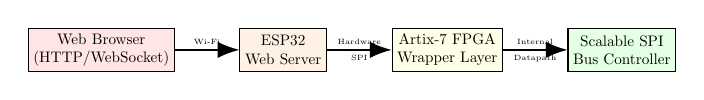
\begin{tikzpicture}[
    scale=0.55, every node/.style={transform shape},
    box/.style={draw, rectangle, minimum height=1cm, minimum width=2cm, align=center, fill=blue!5},
    arrow/.style={draw, -{Latex[scale=1.2]}, thick}
]
    \node [box, fill=red!10] (web) {Web Browser\\(HTTP/WebSocket)};
    \node [box, right=of web, fill=orange!10, xshift=0.5cm] (esp) {ESP32\\Web Server};
    \node [box, right=of esp, fill=yellow!10, xshift=0.5cm] (fpga) {Artix-7 FPGA\\Wrapper Layer};
    \node [box, right=of fpga, fill=green!10, xshift=0.5cm] (bus) {Scalable SPI\\Bus Controller};

    \path [arrow] (web) -- node[above, font=\tiny] {Wi-Fi} (esp);
    \path [arrow] (esp) -- node[above, font=\tiny] {Hardware} node[below, font=\tiny] {SPI} (fpga);
    \path [arrow] (fpga) -- node[above, font=\tiny] {Internal} node[below, font=\tiny] {Datapath} (bus);
    
\end{tikzpicture}
\caption{Web Interface Integration Flow.}
\label{fig:web_interface}
\end{figure}

The ESP32 runs an asynchronous HTTP web server. Users connect to the web interface to select a target sensor address, choose a transaction type (Read/Write), and enter payload data. Upon receiving a command, the ESP32 acts as the SPI master, executing the SPI protocol and transmitting the bits to the FPGA over physical PMOD headers.

\subsection{Web Dashboard Interface Layout and Web Analyzer}
The user interface is a responsive, web-based dashboard styled with clean CSS and an HTML5 Canvas logic analyzer engine. It displays real-time FPGA register states, interactive control fields, signal telemetry, and an automated sequence generator. A high-resolution capture of the live web interface overview is shown in Fig. \ref{fig:web_dashboard_overview}.

\begin{figure}[htbp]
\centering
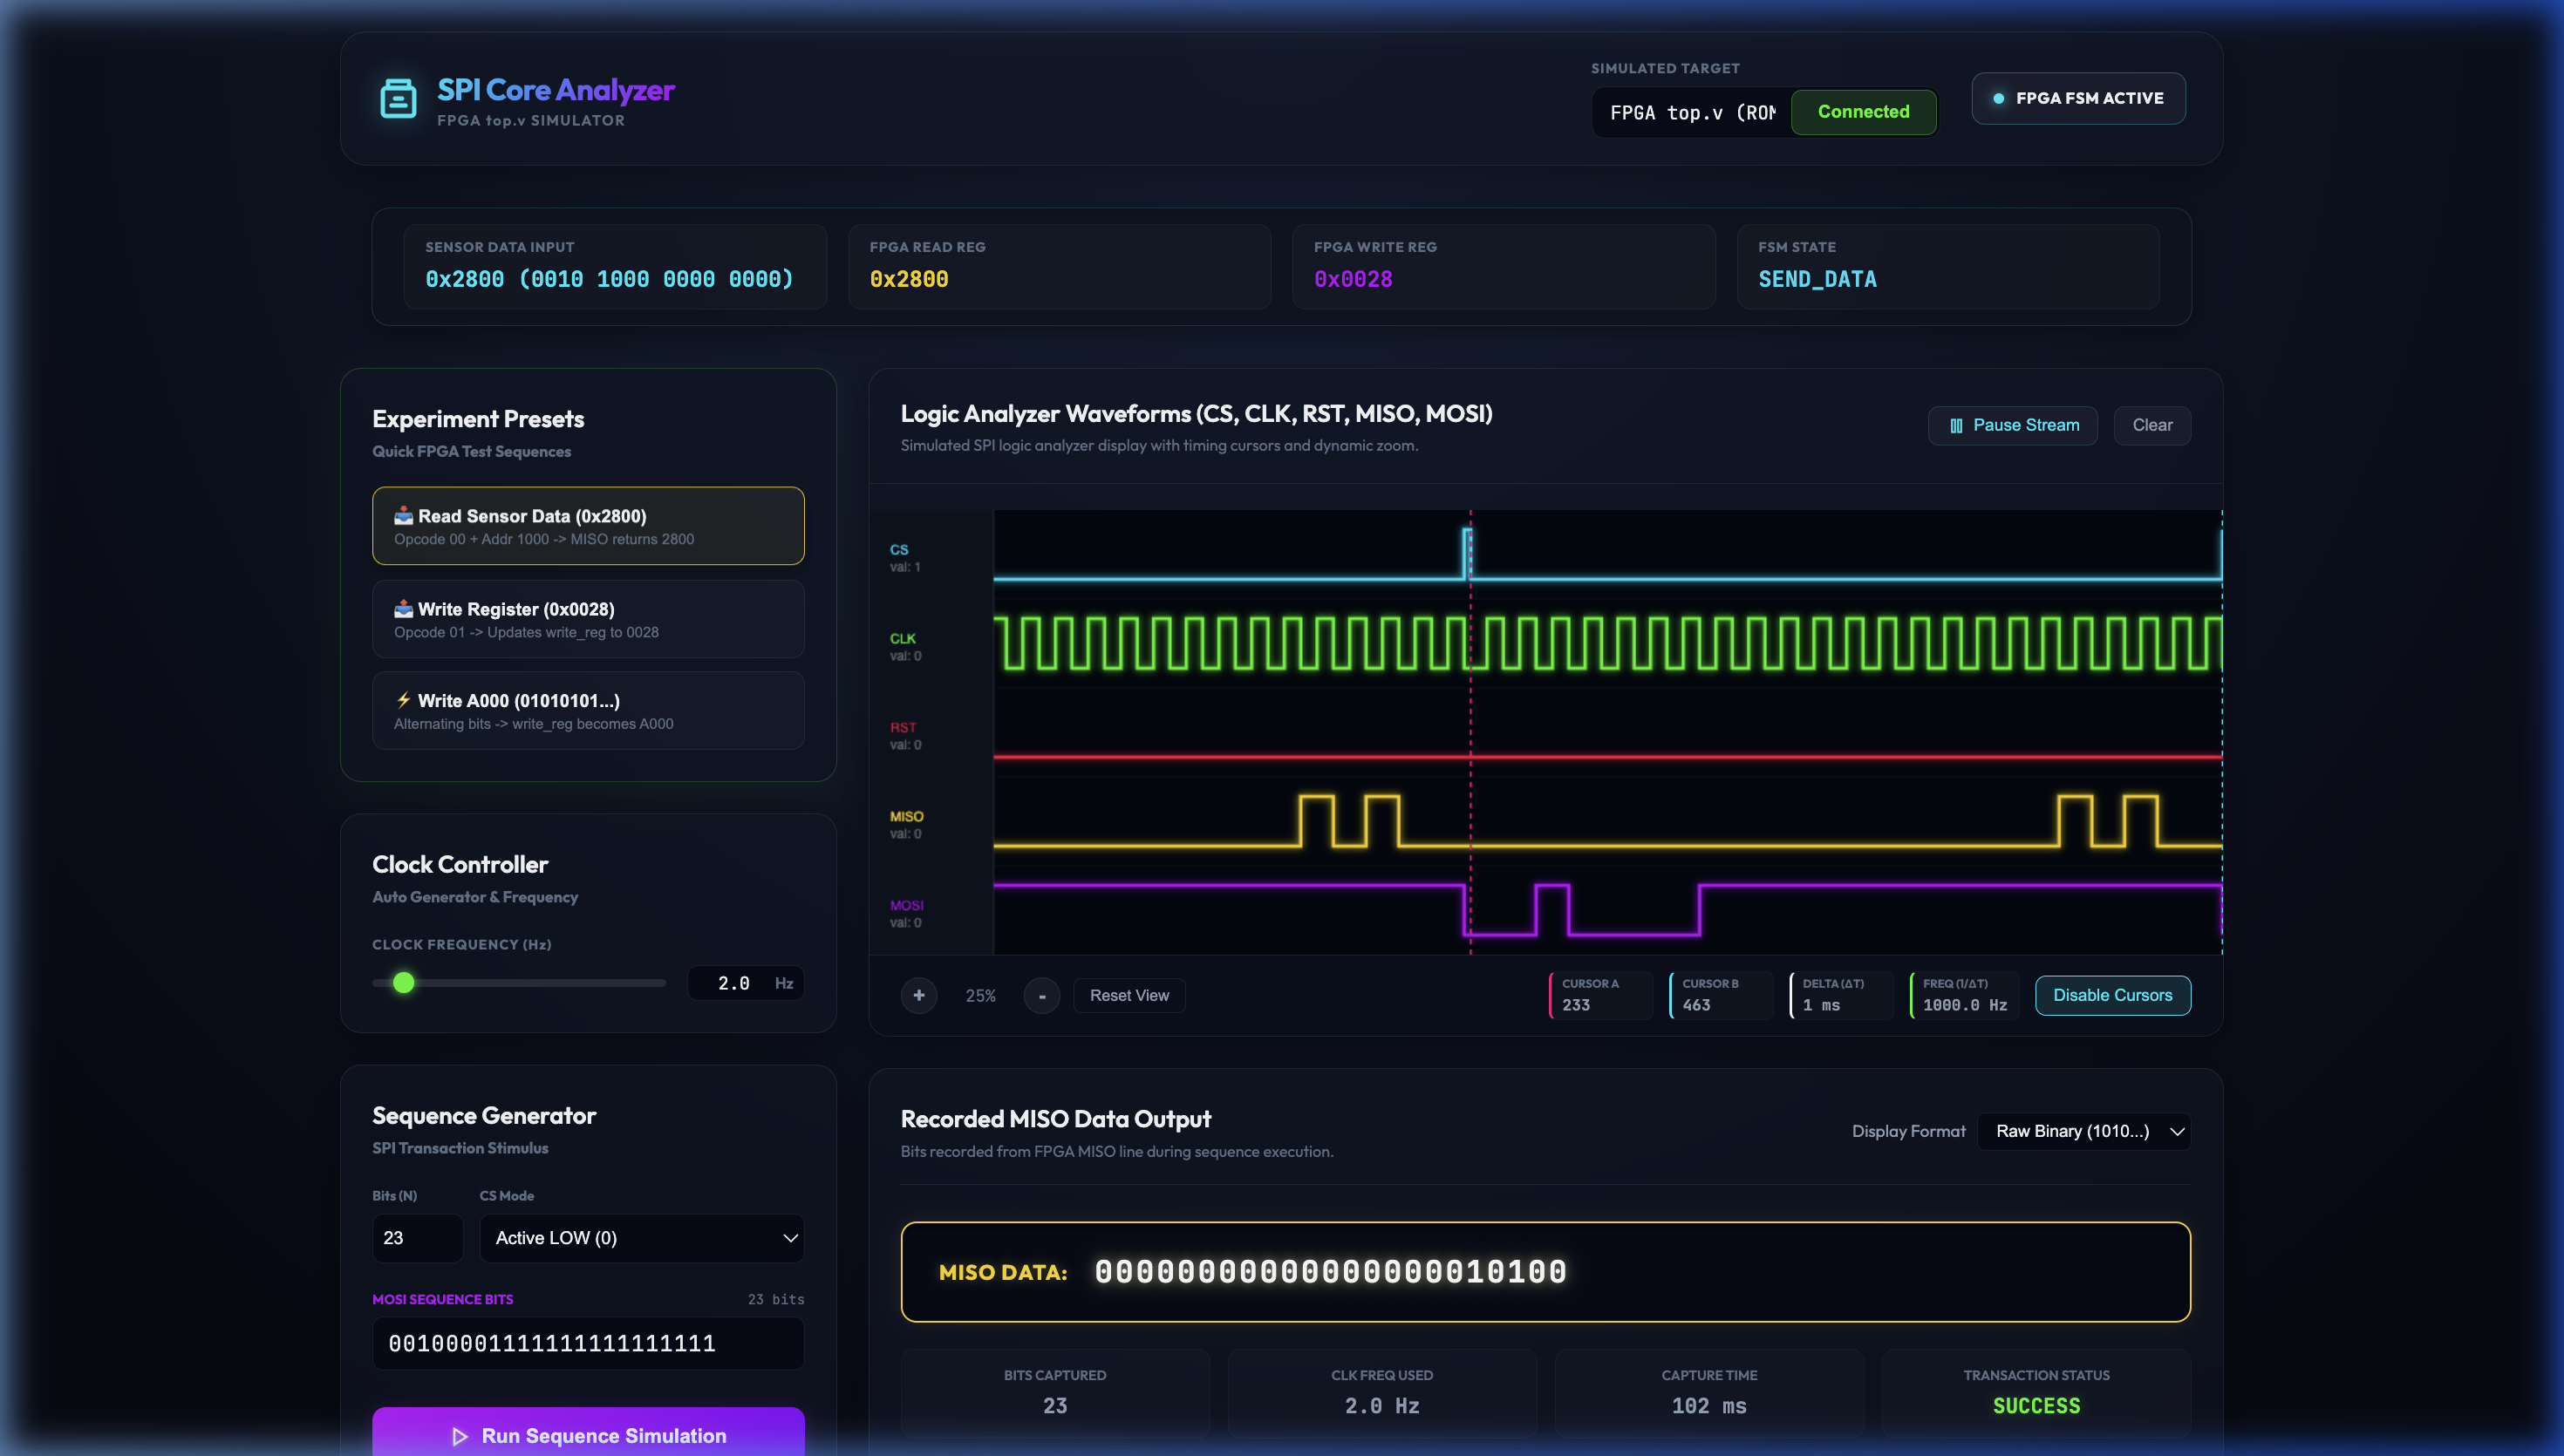
\includegraphics[width=\linewidth]{images/sim_dashboard_overview.png}
\caption{Web Analyzer Dashboard showing the FPGA top.v status banner (\texttt{sensor\_data}, \texttt{read\_reg}, \texttt{write\_reg}, FSM state), interactive quick presets, sequence generator, and live Canvas logic analyzer waveform display.}
\label{fig:web_dashboard_overview}
\end{figure}

The web interface connects directly to the ESP32 backend via REST API endpoints (\texttt{/api/control}, \texttt{/api/sequence}) and receives live telemetry at $20\text{ Hz}$ through a Server-Sent Events (SSE) stream (\texttt{/api/stream}). In addition, an on-board JavaScript simulator implements the exact 9-state FSM of \texttt{top.v}, allowing users to simulate hardware transactions with one-click presets even when physical hardware is disconnected.

\section{Experimental Results and Performance Comparison}
Both SPI protocols were verified using simulation testbenches in Vivado, physical logic analyzer captures connected directly to the FPGA I/O headers, and web-based transaction simulations matching the \texttt{top.v} FSM.

\subsection{Functional Verification and Hardware Signal Capture}
Hardware measurements confirmed accurate bit-level transactions across multiple clock rates and operational modes.

\subsubsection{\texttt{WHO\_AM\_I} State Clock Frequency Tests}
The newly introduced \texttt{WHO\_AM\_I\_STATE} (Opcode \texttt{2'b11}) was subjected to frequency scaling tests to verify clock domain robustness. Logic analyzer traces were captured at both a high-speed $10\text{ MHz}$ SCLK frequency (Fig. \ref{fig:whoami_10m}) and a low-speed $50\text{ kHz}$ SCLK frequency (Fig. \ref{fig:whoami_50k}). 

\begin{figure}[htbp]
\centering
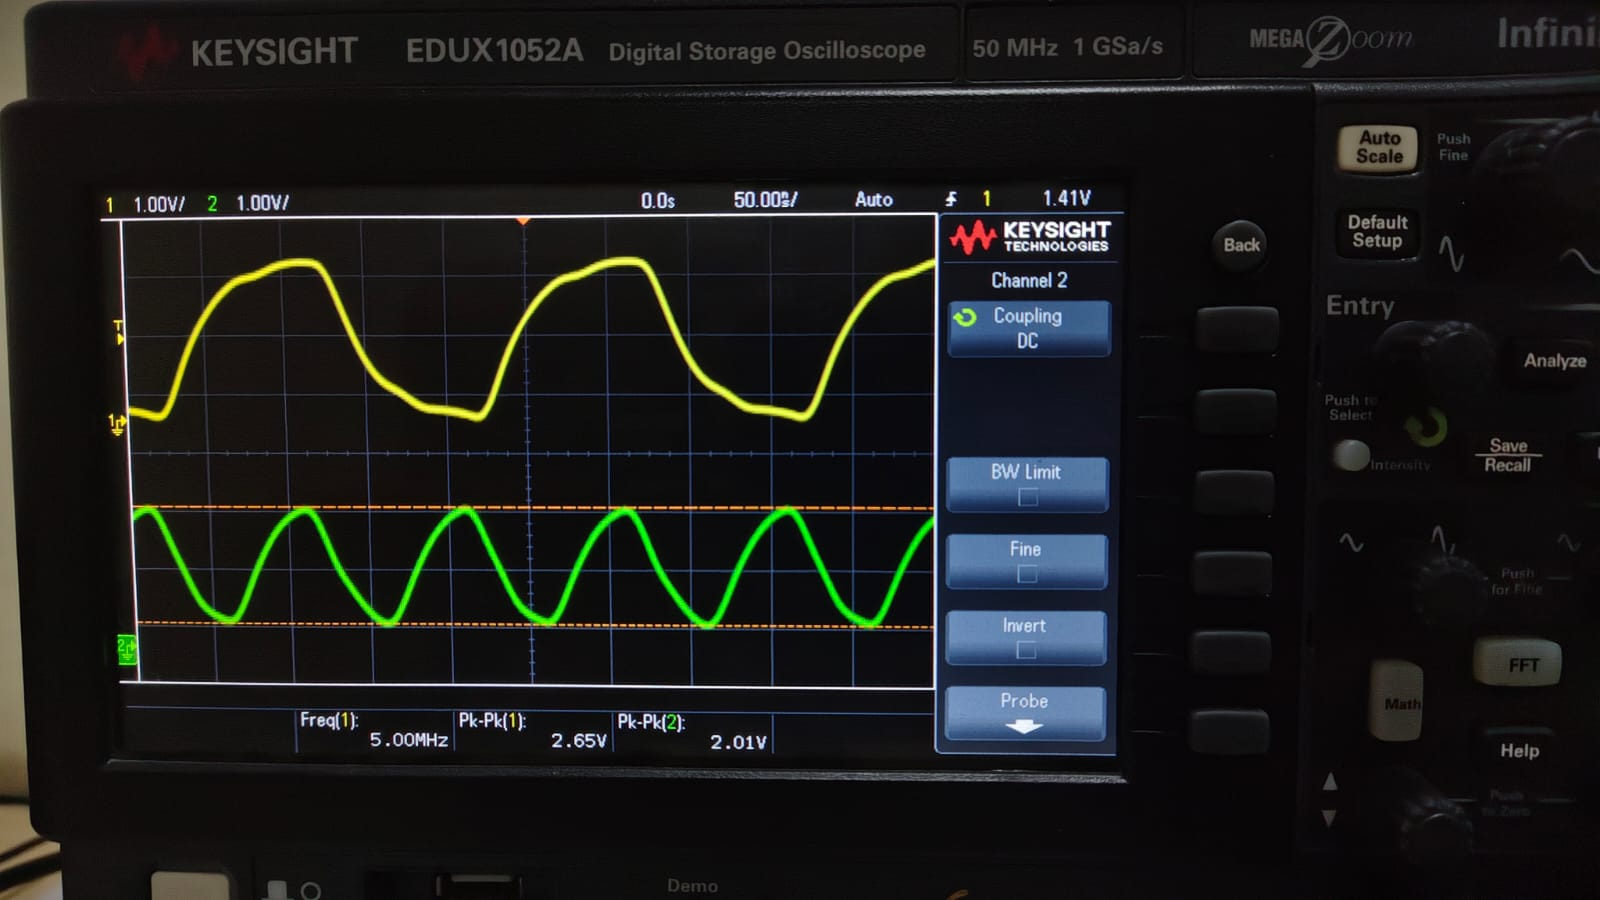
\includegraphics[width=\linewidth]{images/10Mclk-whoami.jpeg}
\caption{Logic analyzer waveform of the \texttt{WHO\_AM\_I} transaction running at $10\text{ MHz}$ clock frequency. The FSM correctly outputs the 8-bit sensor identifier (\texttt{SENSOR\_ID = 8'd9}) on MISO.}
\label{fig:whoami_10m}
\end{figure}

\begin{figure}[htbp]
\centering
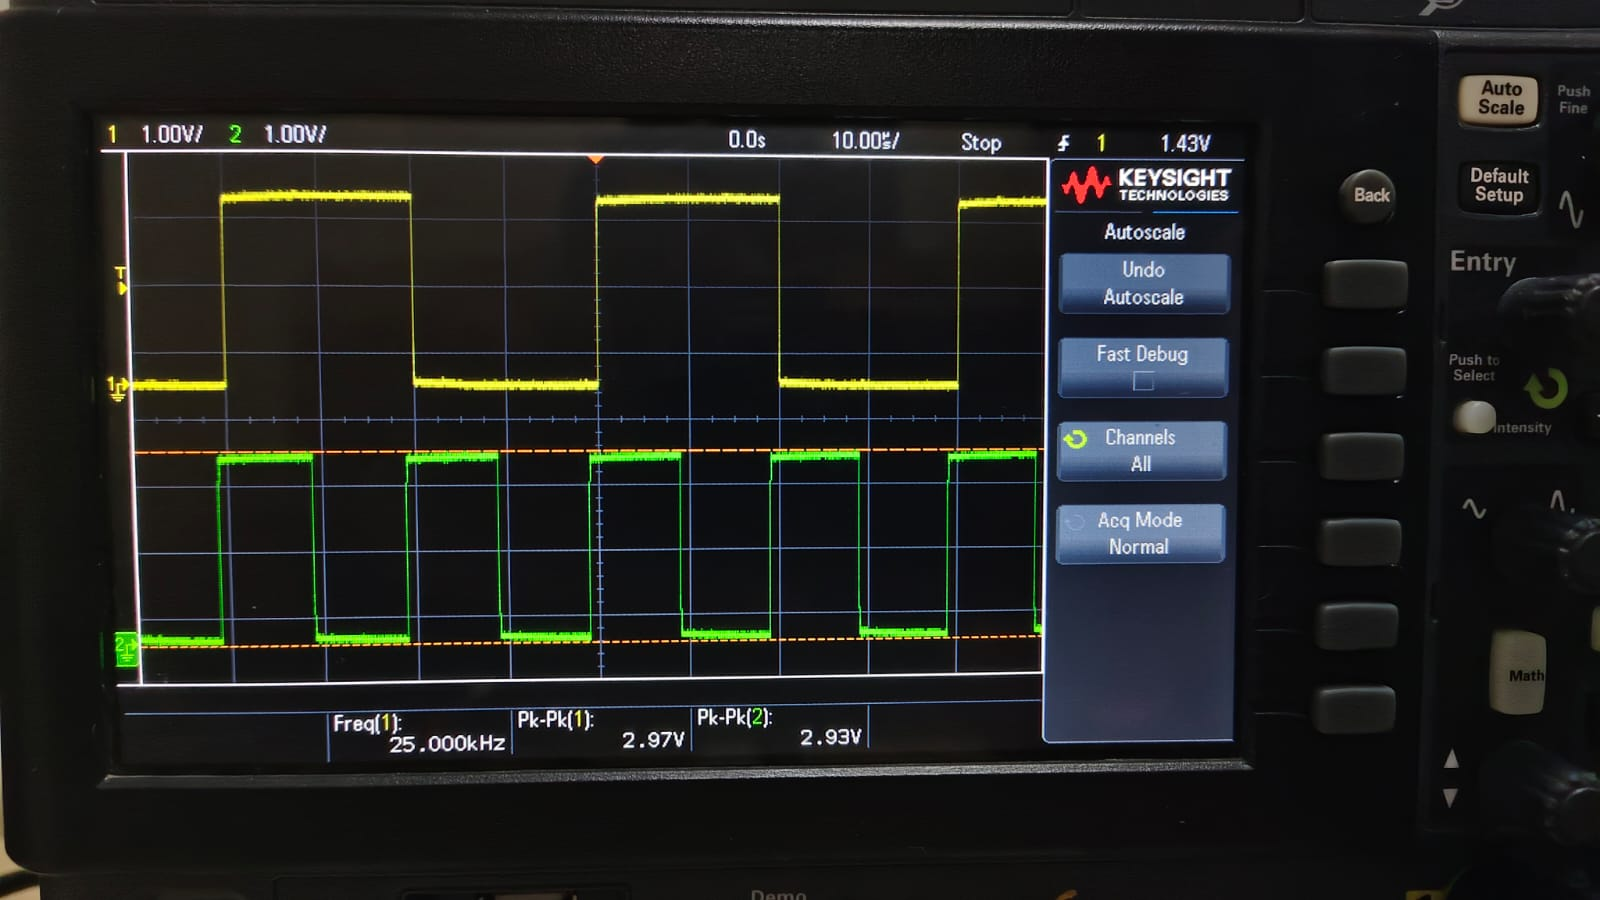
\includegraphics[width=\linewidth]{images/50khz_clk-whoami.jpeg}
\caption{Logic analyzer waveform of the \texttt{WHO\_AM\_I} transaction running at $50\text{ kHz}$ clock frequency, confirming reliable operation across wide frequency ranges.}
\label{fig:whoami_50k}
\end{figure}

As seen in the waveform captures, the FSM decodes opcode \texttt{2'b11} in state \texttt{DETECT} and immediately transitions to \texttt{WHO\_AM\_I\_STATE}, shifting out the 8-bit \texttt{SENSOR\_ID} parameter on MISO over 8 clock cycles. The timing captures confirm zero setup/hold timing violations or missing bits across frequencies from $50\text{ kHz}$ up to $10\text{ MHz}$.

\subsubsection{Oscilloscope and Signal Capture Analysis}
Fig. \ref{fig:read_sensor} and Fig. \ref{fig:read_mosi_miso} present logic analyzer captures for MOSI command transmission and MISO data reception.

\begin{figure}[htbp]
\centering
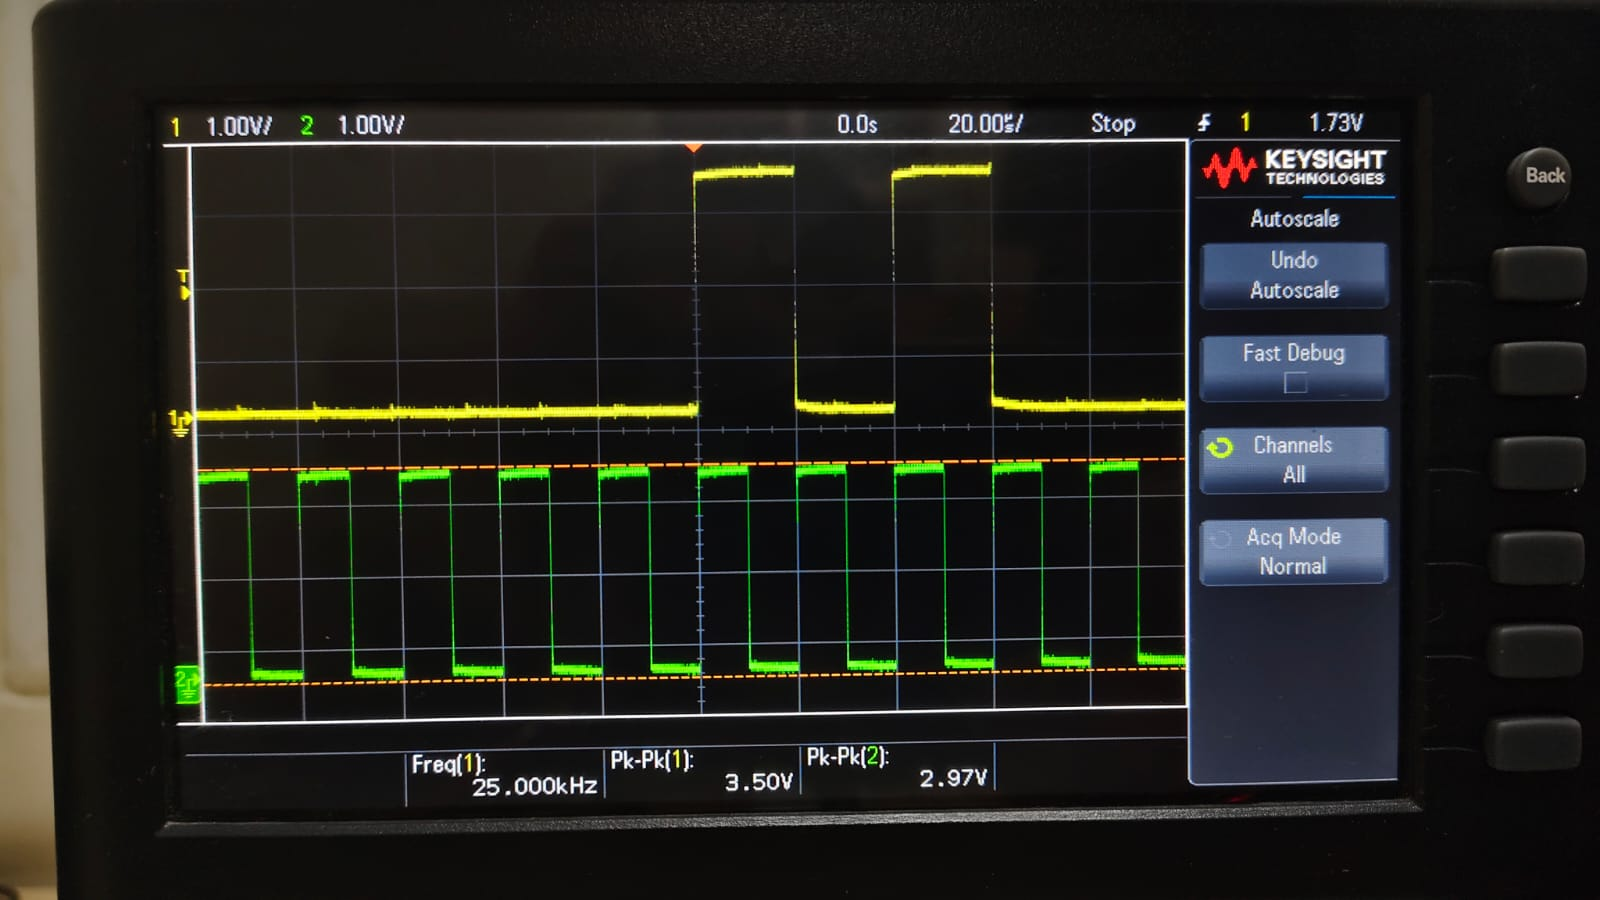
\includegraphics[width=\linewidth]{images/50khz_clk_read_sensor_A.jpeg}
\caption{Logic analyzer capture of a Sensor Read operation at $50\text{ kHz}$ SCLK, verifying accurate data retrieval from parallel DIP switch inputs onto MISO.}
\label{fig:read_sensor}
\end{figure}

\begin{figure}[htbp]
\centering
\subfloat[MOSI Read Command]{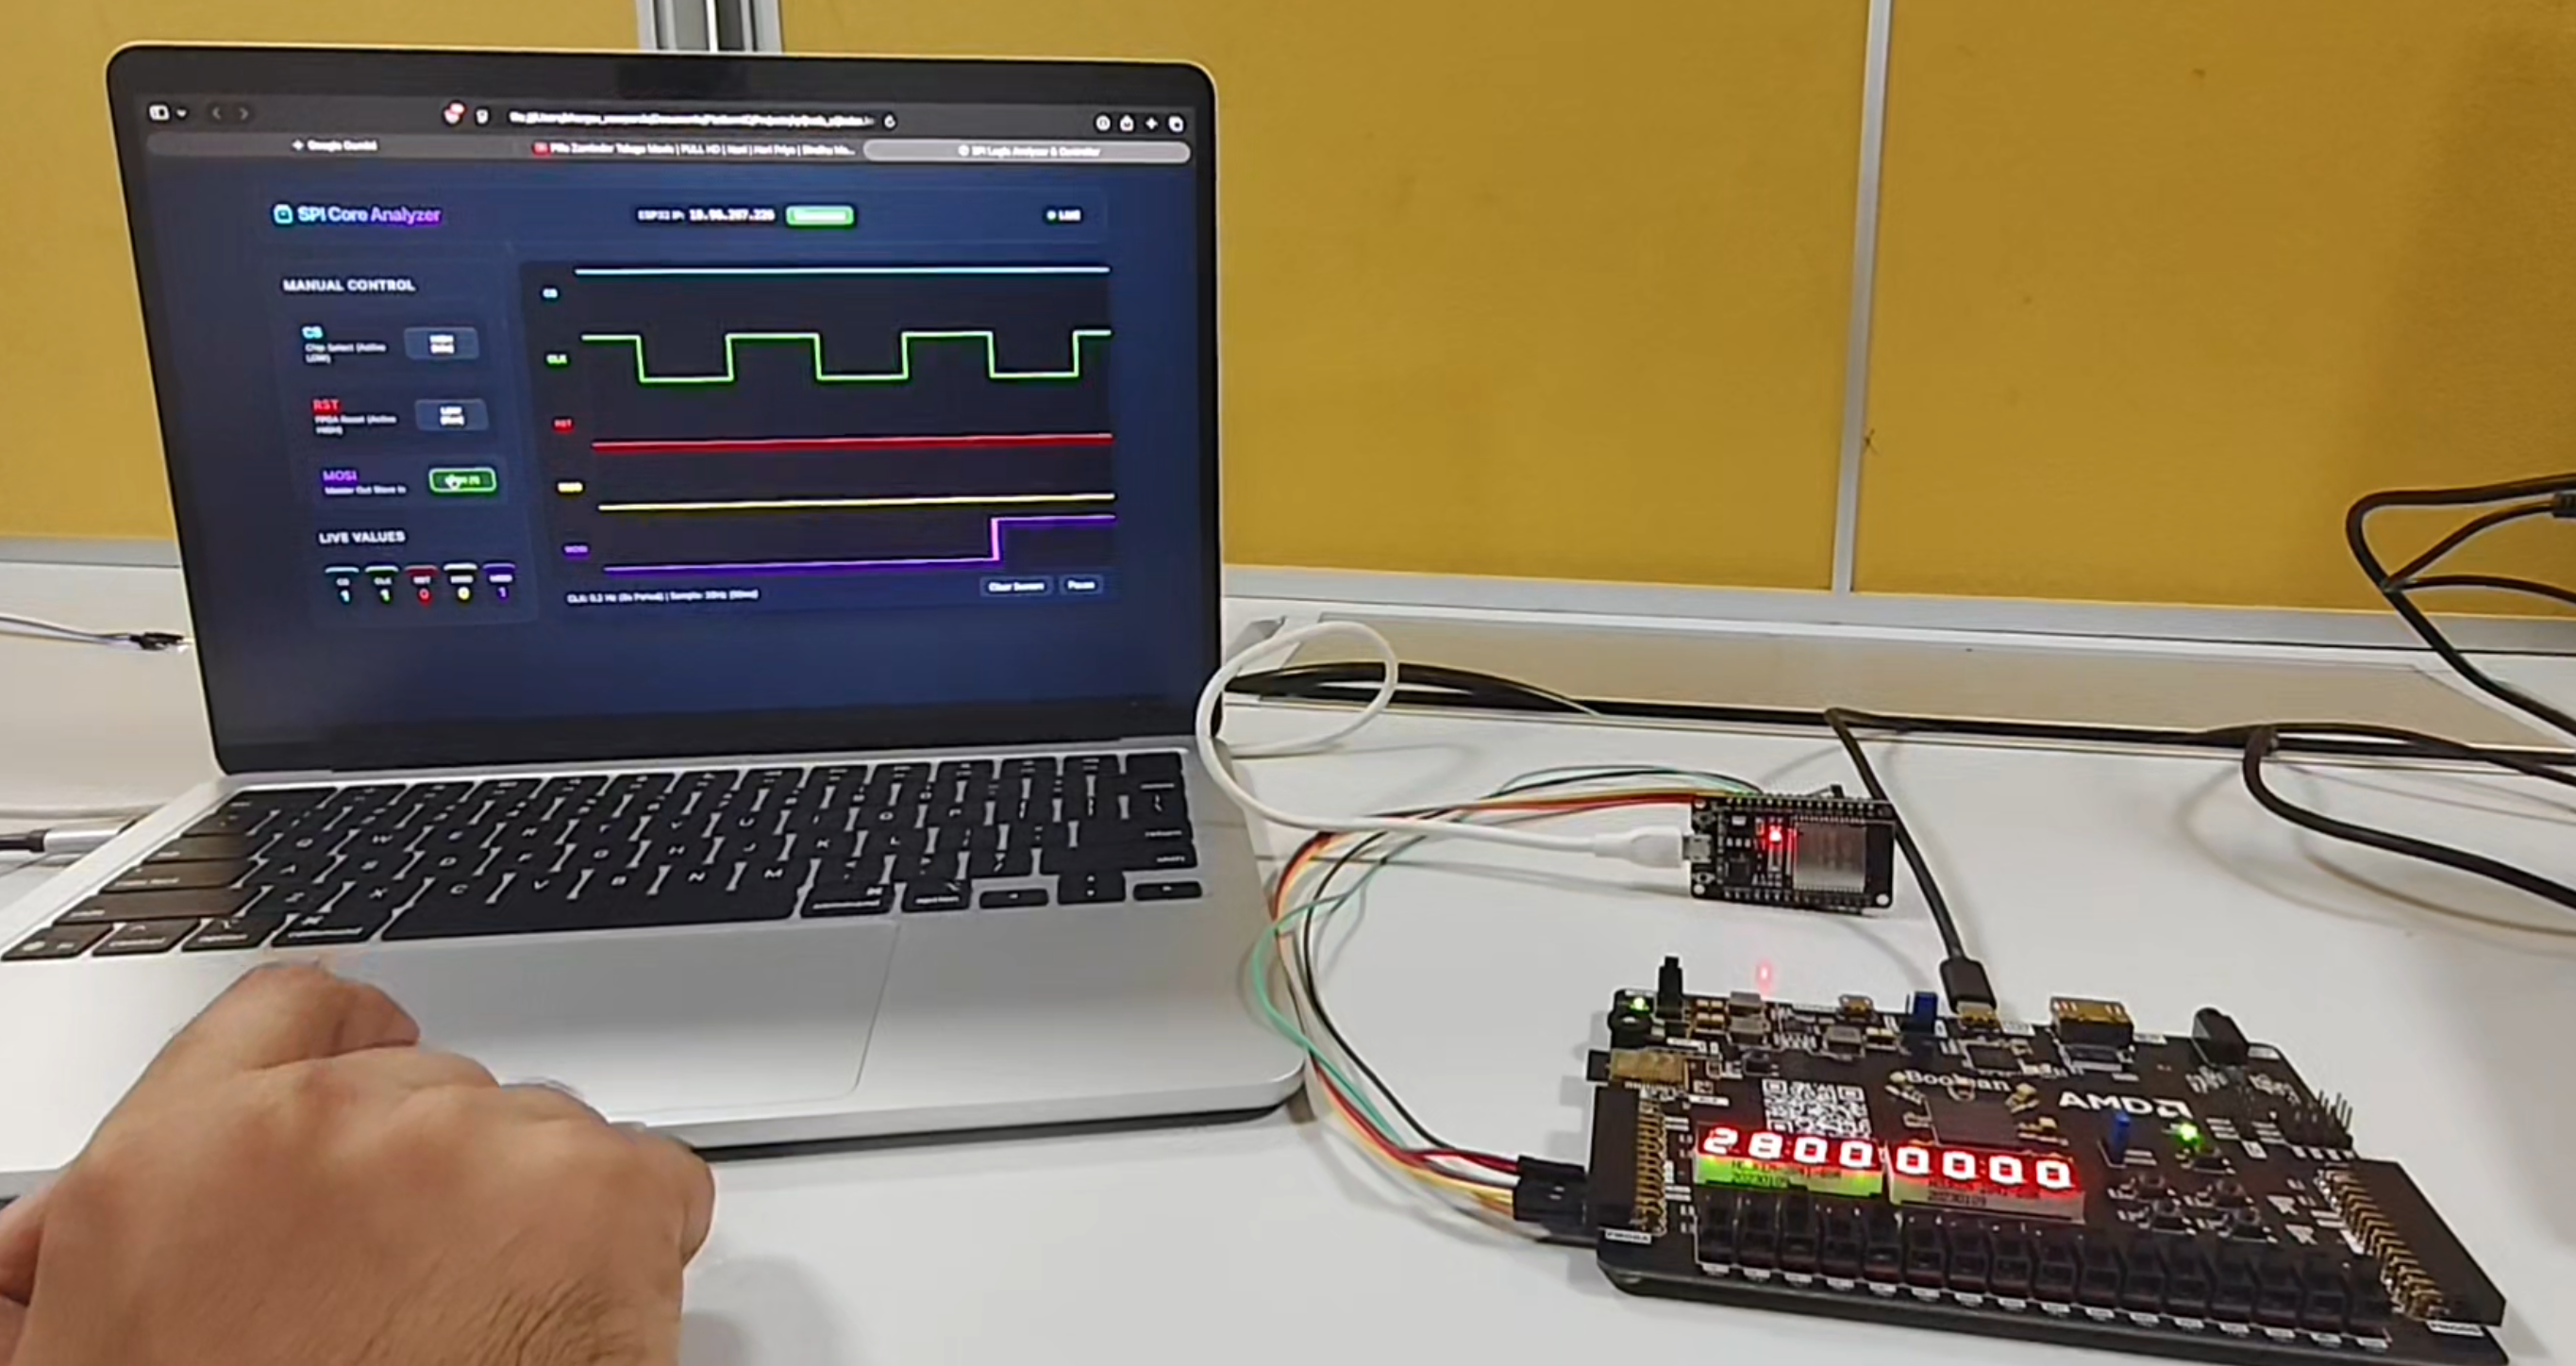
\includegraphics[width=0.48\linewidth]{images/asking_read_MOSI.png}\label{fig:read_mosi}}\hfill
\subfloat[MISO Read Response]{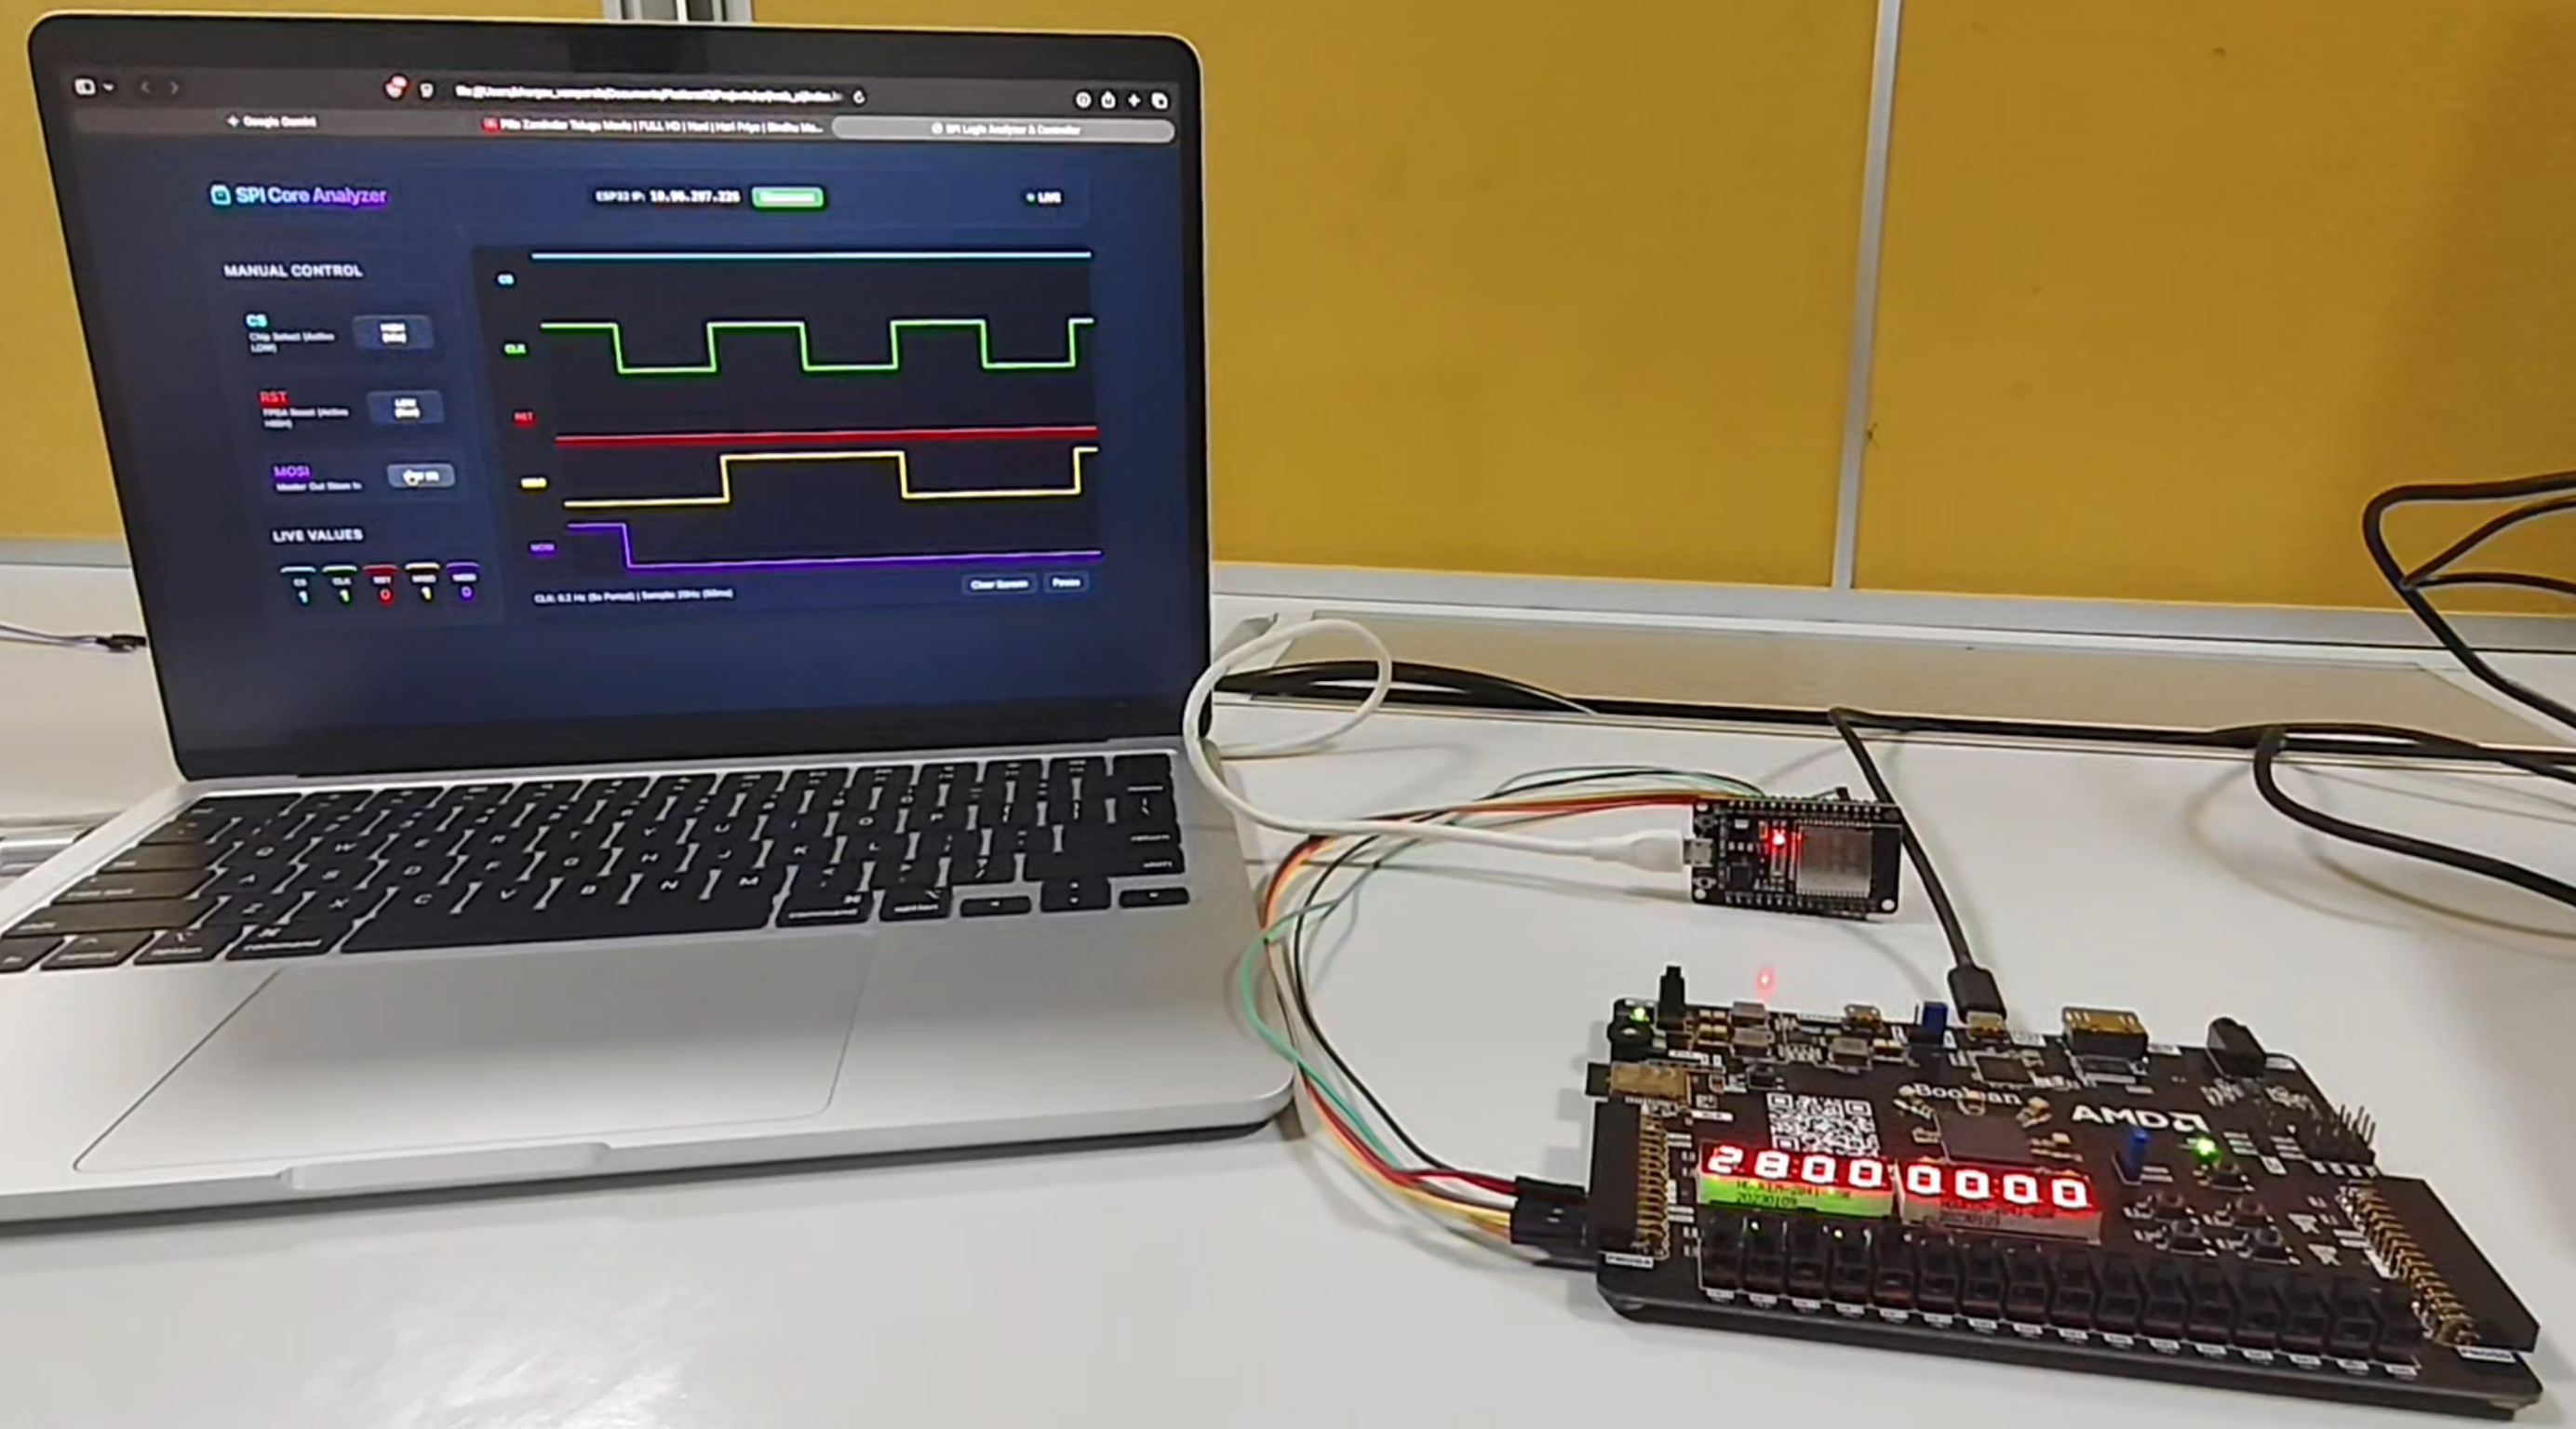
\includegraphics[width=0.48\linewidth]{images/reciving_read_MISO.png}\label{fig:read_miso}}
\caption{Oscilloscope captures showing (a) MOSI command transmission requesting register read, and (b) corresponding MISO response streaming from the FPGA.}
\label{fig:read_mosi_miso}
\end{figure}

\begin{figure}[htbp]
\centering
\subfloat[Write Sequence Start]{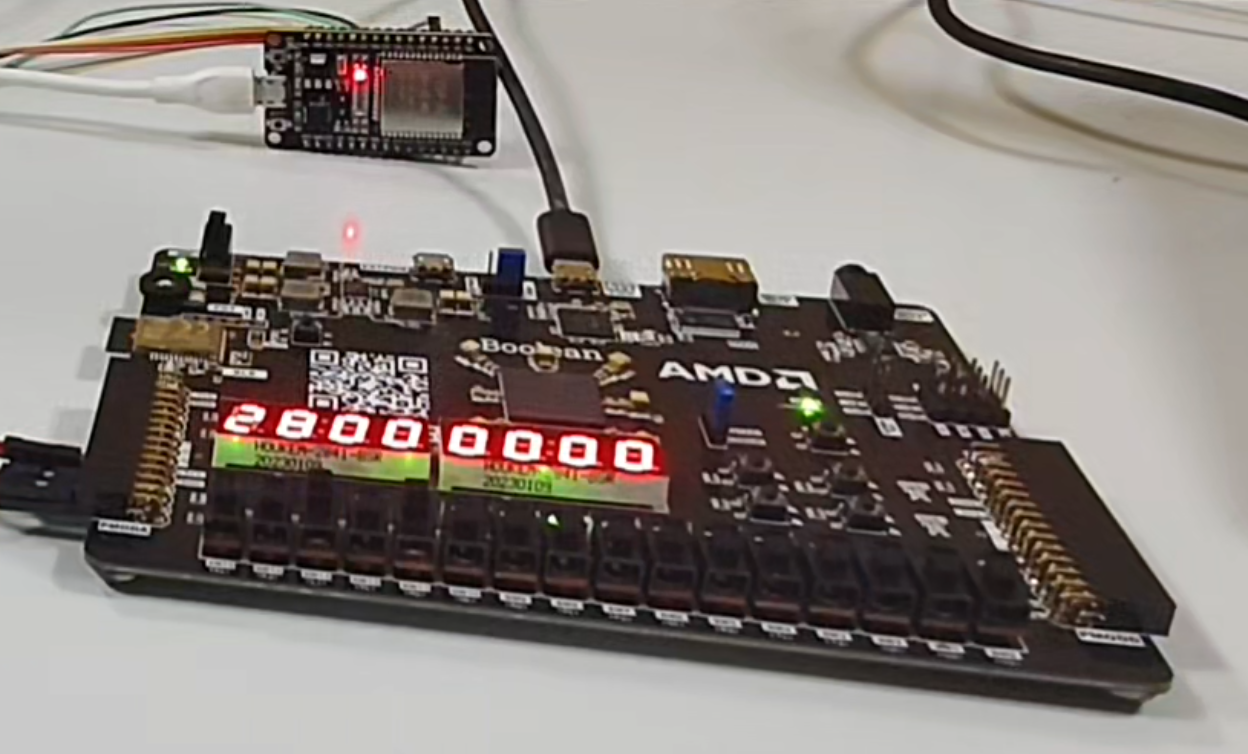
\includegraphics[width=0.48\linewidth]{images/write-1.png}\label{fig:write_1}}\hfill
\subfloat[Write Payload Transfer]{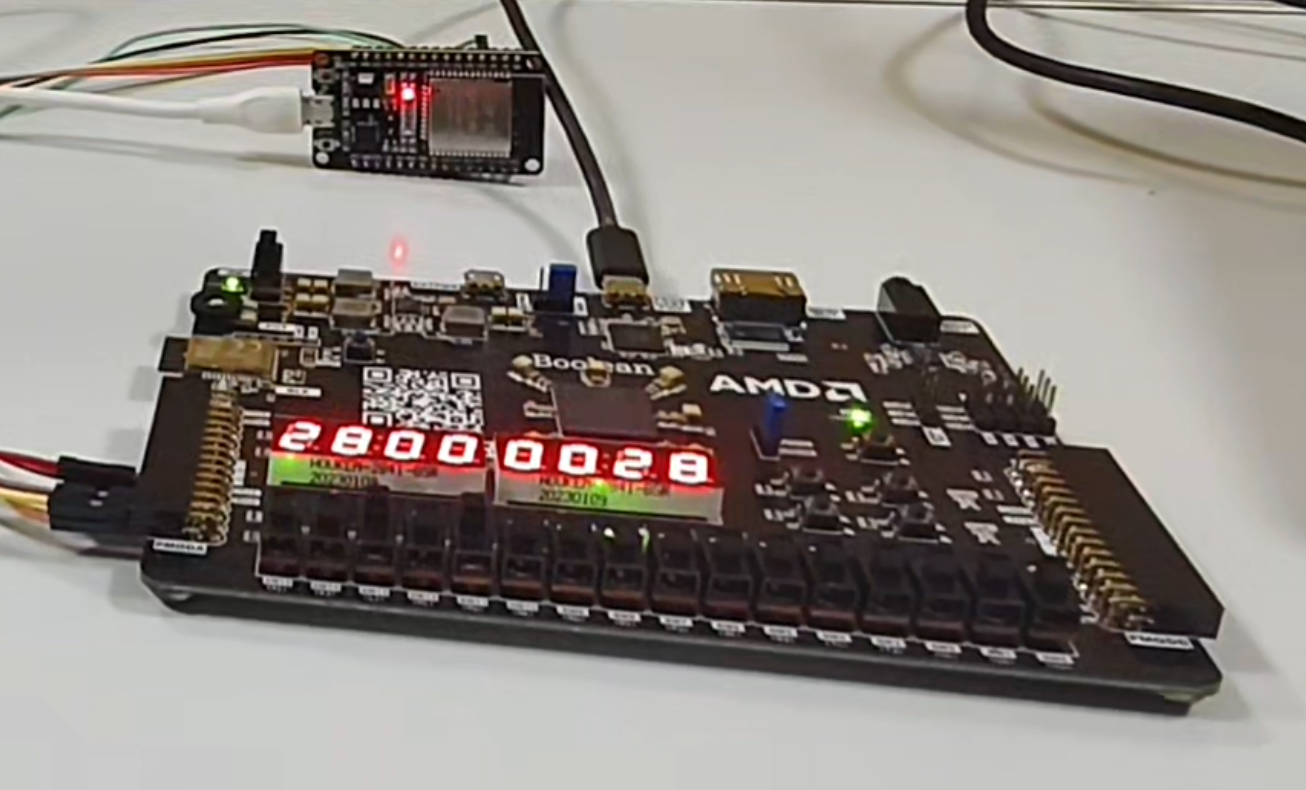
\includegraphics[width=0.48\linewidth]{images/write-2.png}\label{fig:write_2}}
\caption{Oscilloscope captures showing write transaction execution on MOSI and MISO signals.}
\label{fig:write_oscilloscope}
\end{figure}


\subsection{Verification Case Studies and Simulation Analysis}

To validate system behavior across complex data patterns, three primary test cases were evaluated:

\subsubsection{Case Study 1: Sensor Data Read (\texttt{0x2800})}
In Case Study 1, the physical sensor input is configured with \texttt{sensor\_data = 16'h2800} (binary: \texttt{0010 1000 0000 0000}). The master executes a Read command by sending opcode \texttt{00} followed by address \texttt{1000} (address 16, mapping to \texttt{read\_reg}) and 16 clock cycles with MOSI = \texttt{0}.

\begin{figure}[htbp]
\centering
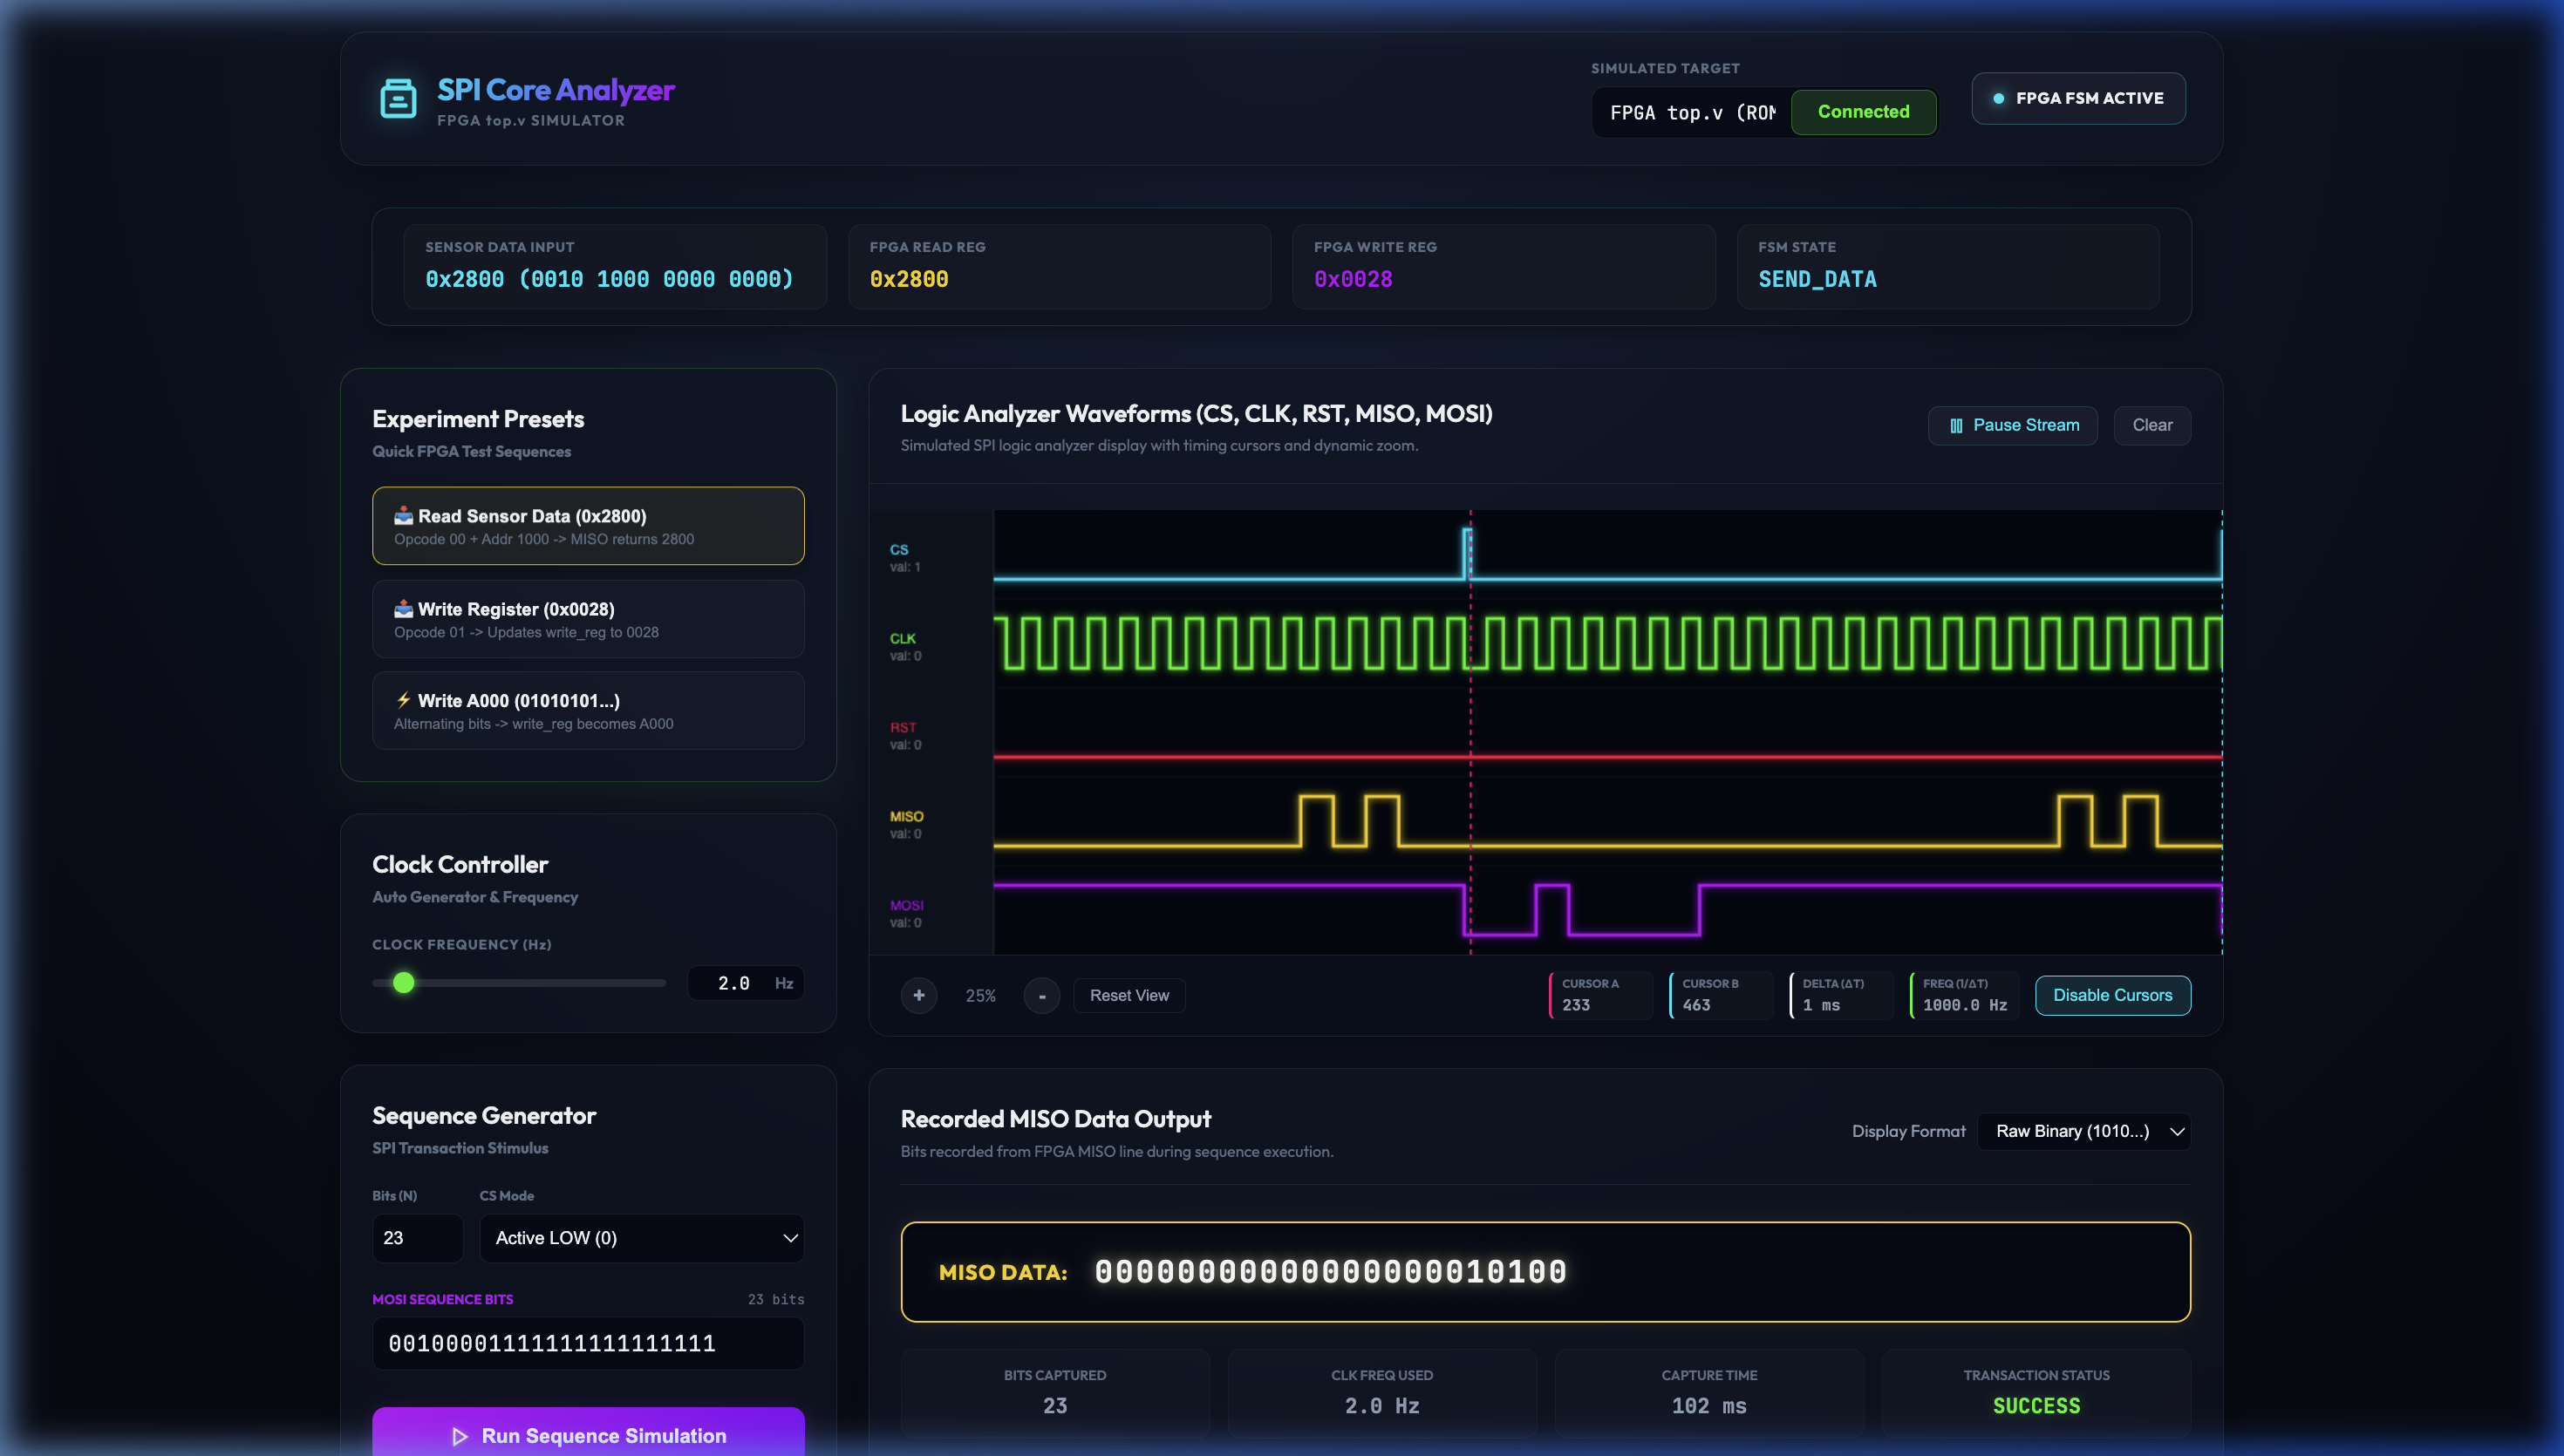
\includegraphics[width=\linewidth]{images/sim_read_2800.png}
\caption{Web Analyzer simulation of Sensor Data Read (\texttt{0x2800}). The MISO recorded data output displays \texttt{0010100000000000} (\texttt{0x2800} in Hex).}
\label{fig:sim_read_2800}
\end{figure}

Table \ref{tab:bit_read_2800} provides the bit-by-bit parsing analysis for the Read \texttt{0x2800} transaction across 22 clock cycles.

\begin{table}[htbp]
\caption{Bit-by-Bit Breakdown for Sensor Read Transaction (\texttt{0x2800})}
\label{tab:bit_read_2800}
\centering
\resizebox{\columnwidth}{!}{%
\begin{tabular}{ccllc}
\toprule
\textbf{Cycle} & \textbf{MOSI} & \textbf{FSM State} & \textbf{Operation / Action} & \textbf{MISO Output} \\
\midrule
1 & \texttt{0} & \texttt{DETECT} & \texttt{mode[1] <= 0} & \texttt{0} \\
2 & \texttt{0} & \texttt{DETECT} & \texttt{mode[0] <= 0} $\rightarrow$ Opcode \texttt{00} (READ). \texttt{read\_reg <= 0x2800} & \texttt{0} \\
3..6 & \texttt{1000} & \texttt{READ\_ADDR} & Shifts address bits ($\text{addr} = 16$) & \texttt{0} \\
7 & \texttt{0} & \texttt{SEND\_DATA} & Clocks out Bit 15 (\texttt{0}) & \texttt{0} \\
8 & \texttt{0} & \texttt{SEND\_DATA} & Clocks out Bit 14 (\texttt{0}) & \texttt{0} \\
9 & \texttt{0} & \texttt{SEND\_DATA} & Clocks out Bit 13 (\texttt{1}) & \textbf{\texttt{1}} \\
10 & \texttt{0} & \texttt{SEND\_DATA} & Clocks out Bit 12 (\texttt{0}) & \texttt{0} \\
11 & \texttt{0} & \texttt{SEND\_DATA} & Clocks out Bit 11 (\texttt{1}) & \textbf{\texttt{1}} \\
12..22 & \texttt{0...} & \texttt{SEND\_DATA} & Clocks out remaining lower bits (\texttt{0000 0000 0000}) & \texttt{0} \\
\bottomrule
\end{tabular}%
}
\end{table}

As shown in Table \ref{tab:bit_read_2800} and Fig. \ref{fig:sim_read_2800}, MISO streams \texttt{0010100000000000}, accurately recovering the sensor value \texttt{0x2800}.

\subsubsection{Case Study 2: Register Write (\texttt{0x0028})}
In Case Study 2, the master writes payload data to update \texttt{write\_reg} from \texttt{0x0000} to \texttt{16'h0028} (binary: \texttt{0000 0000 0010 1000}). The transaction sends opcode \texttt{01} (WRITE), address \texttt{0000}, write length \texttt{0101} ($5 \implies 6$ data bits), and data bits \texttt{001010} (setting bit 3 and bit 5 to \texttt{1}).

\begin{figure}[htbp]
\centering
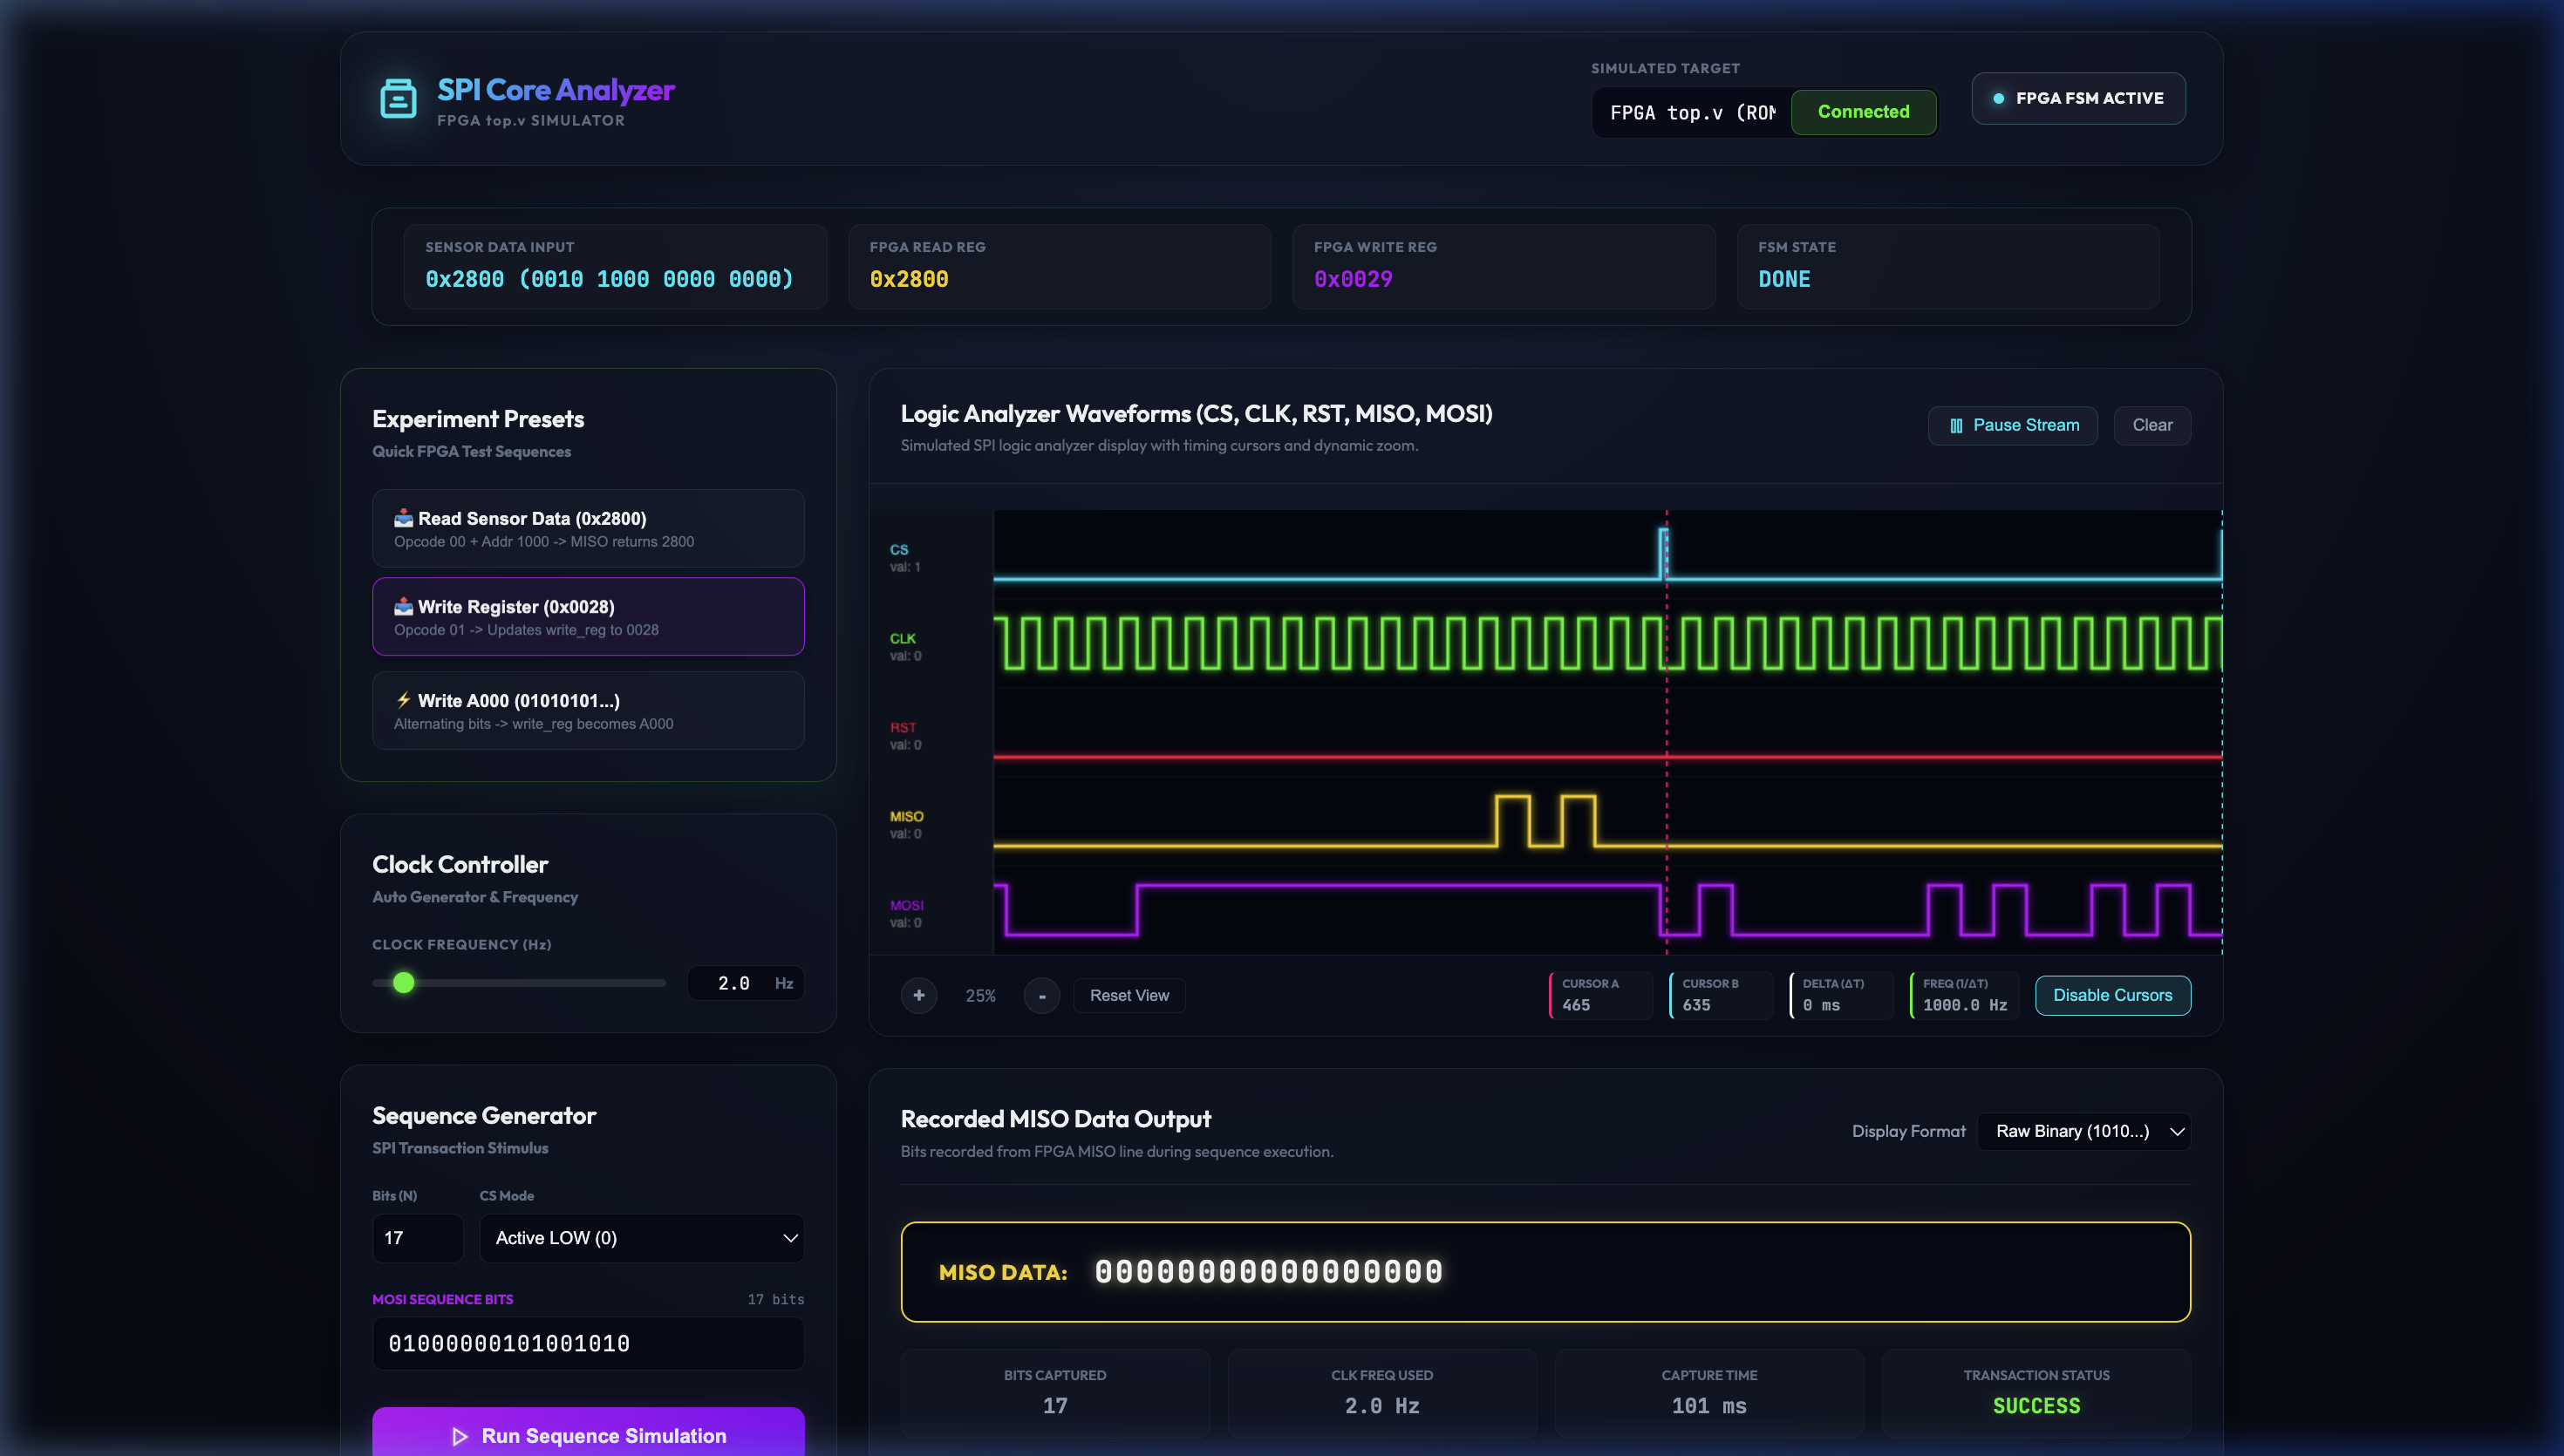
\includegraphics[width=\linewidth]{images/sim_write_0028.png}
\caption{Web Analyzer simulation of Register Write (\texttt{0x0028}). \texttt{write\_reg} is successfully updated to \texttt{0x0028}.}
\label{fig:sim_write_0028}
\end{figure}

Table \ref{tab:bit_write_0028} outlines the cycle-by-cycle bit parsing for the Write \texttt{0x0028} transaction.

\begin{table}[htbp]
\caption{Bit-by-Bit Breakdown for Register Write Transaction (\texttt{0x0028})}
\label{tab:bit_write_0028}
\centering
\resizebox{\columnwidth}{!}{%
\begin{tabular}{ccllc}
\toprule
\textbf{Cycle} & \textbf{MOSI} & \textbf{FSM State} & \textbf{Operation / Action} & \textbf{write\_reg State} \\
\midrule
1 & \texttt{0} & \texttt{DETECT} & \texttt{mode[1] <= 0} & \texttt{0x0000} \\
2 & \texttt{1} & \texttt{DETECT} & \texttt{mode[0] <= 1} $\rightarrow$ Opcode \texttt{01} (WRITE) & \texttt{0x0000} \\
3..6 & \texttt{0000} & \texttt{WRITE\_ADDR} & Sets address $\text{addr} = 0$ & \texttt{0x0000} \\
7..10 & \texttt{0101} & \texttt{WRITE\_LEN} & Sets $\text{write\_len} = 5$ ($6$ data bits) & \texttt{0x0000} \\
11 & \texttt{0} & \texttt{WRITE\_DATA} & Writes bit 0 $\rightarrow$ \texttt{write\_reg[0] = 0} & \texttt{0x0000} \\
12 & \texttt{0} & \texttt{WRITE\_DATA} & Writes bit 1 $\rightarrow$ \texttt{write\_reg[1] = 0} & \texttt{0x0000} \\
13 & \texttt{1} & \texttt{WRITE\_DATA} & Writes bit 2 $\rightarrow$ \texttt{write\_reg[2] = 0} & \texttt{0x0000} \\
14 & \texttt{0} & \texttt{WRITE\_DATA} & Writes bit 3 $\rightarrow$ \texttt{write\_reg[3] = 1} & \texttt{0x0008} \\
15 & \texttt{1} & \texttt{WRITE\_DATA} & Writes bit 4 $\rightarrow$ \texttt{write\_reg[4] = 0} & \texttt{0x0008} \\
16 & \texttt{0} & \texttt{WRITE\_DATA} & Writes bit 5 $\rightarrow$ \texttt{write\_reg[5] = 1} & \textbf{\texttt{0x0028}} \\
\bottomrule
\end{tabular}%
}
\end{table}

\subsubsection{Case Study 3: The 010101 Phenomenon (\texttt{0xA000})}
During physical testing with an unformatted signal stream, an interesting phenomenon was observed: driving a continuous alternating bit pattern (\texttt{0101010101...}) onto the MOSI line while Chip Select (\texttt{cs}) was held low caused an unintentional valid write transaction to Sensor 4 (the 5th sensor entry in the ROM table), updating the 16-bit \texttt{write\_reg} from \texttt{16'h0000} to \texttt{16'hA000}.

The web simulation capture and physical 7-segment display states are shown in Fig. \ref{fig:sim_write_a000} and Fig. \ref{fig:phenomenon_display}.

\begin{figure}[htbp]
\centering
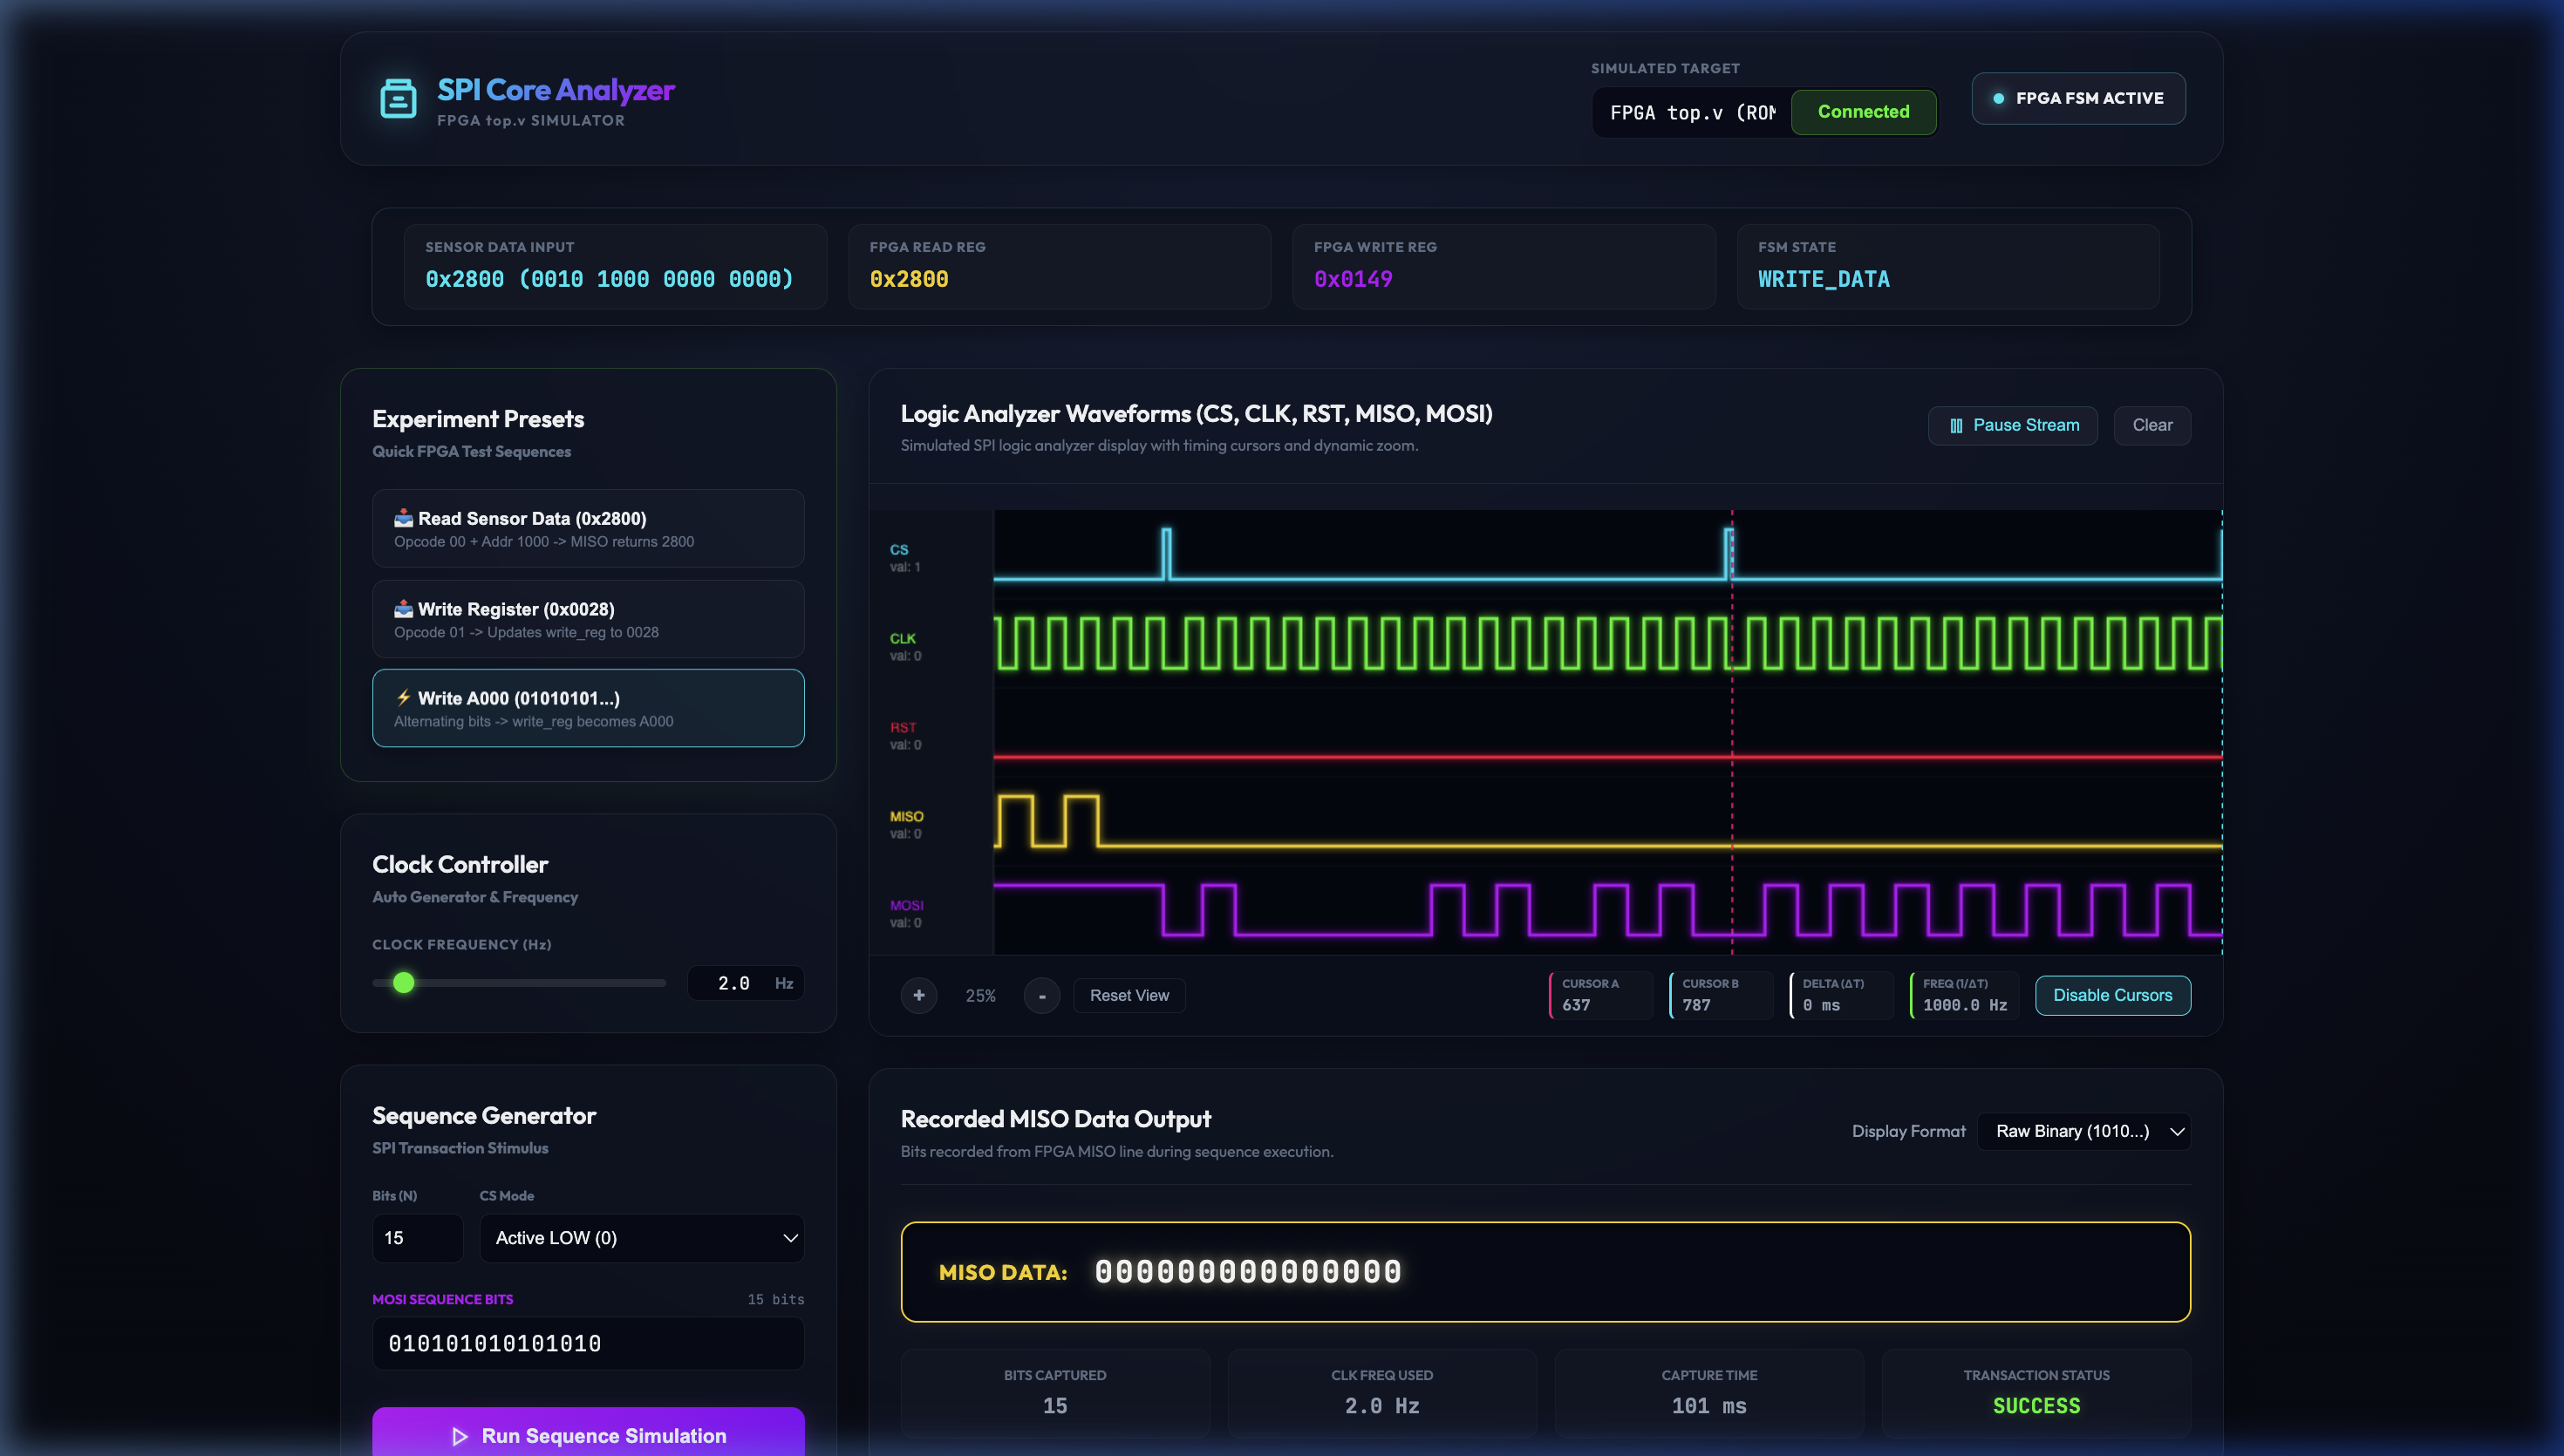
\includegraphics[width=\linewidth]{images/sim_write_a000.png}
\caption{Web Analyzer simulation of the alternating \texttt{01010101...} sequence updating \texttt{write\_reg} to \texttt{0xA000}.}
\label{fig:sim_write_a000}
\end{figure}

\begin{figure}[htbp]
\centering
\subfloat[Initial Display State (0000)]{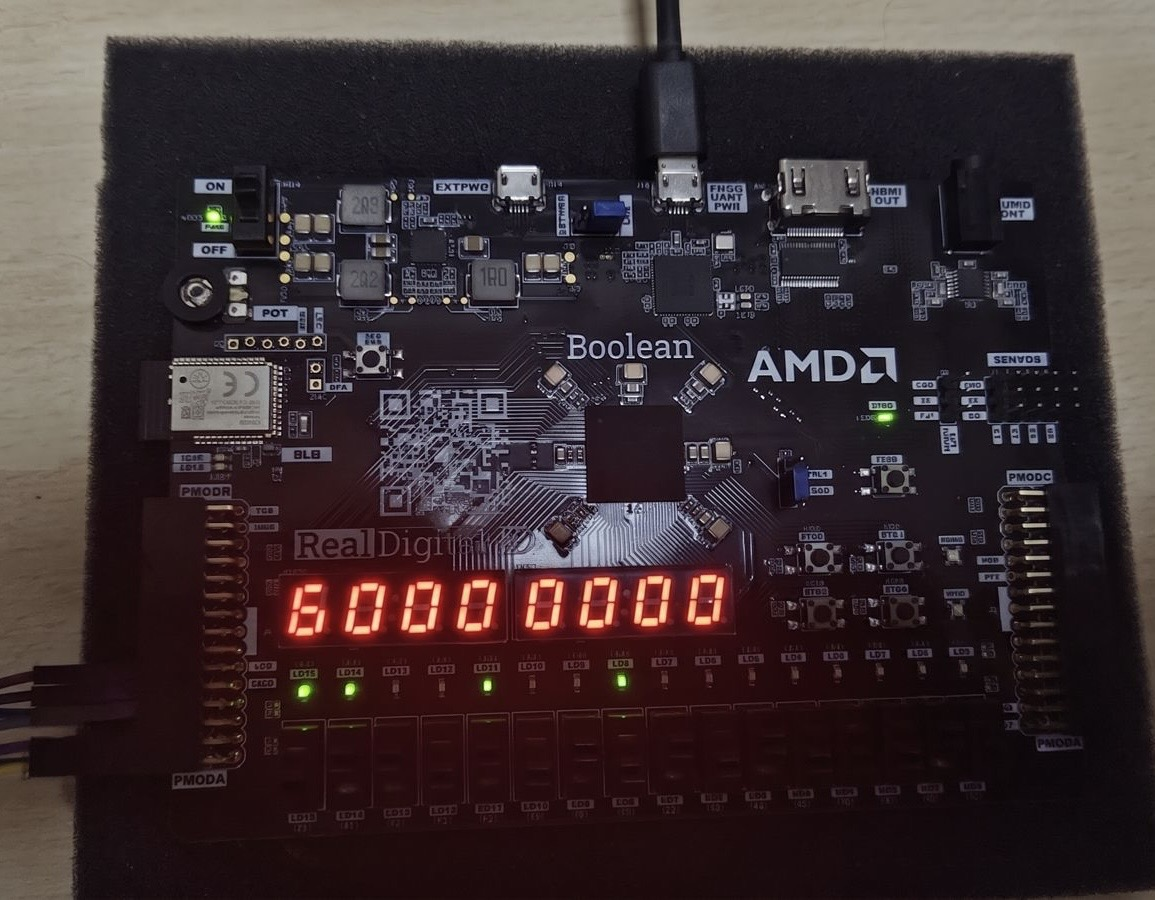
\includegraphics[width=0.48\linewidth]{images/0000.jpg}\label{fig:disp_0000}}\hfill
\subfloat[Updated Display State (A000)]{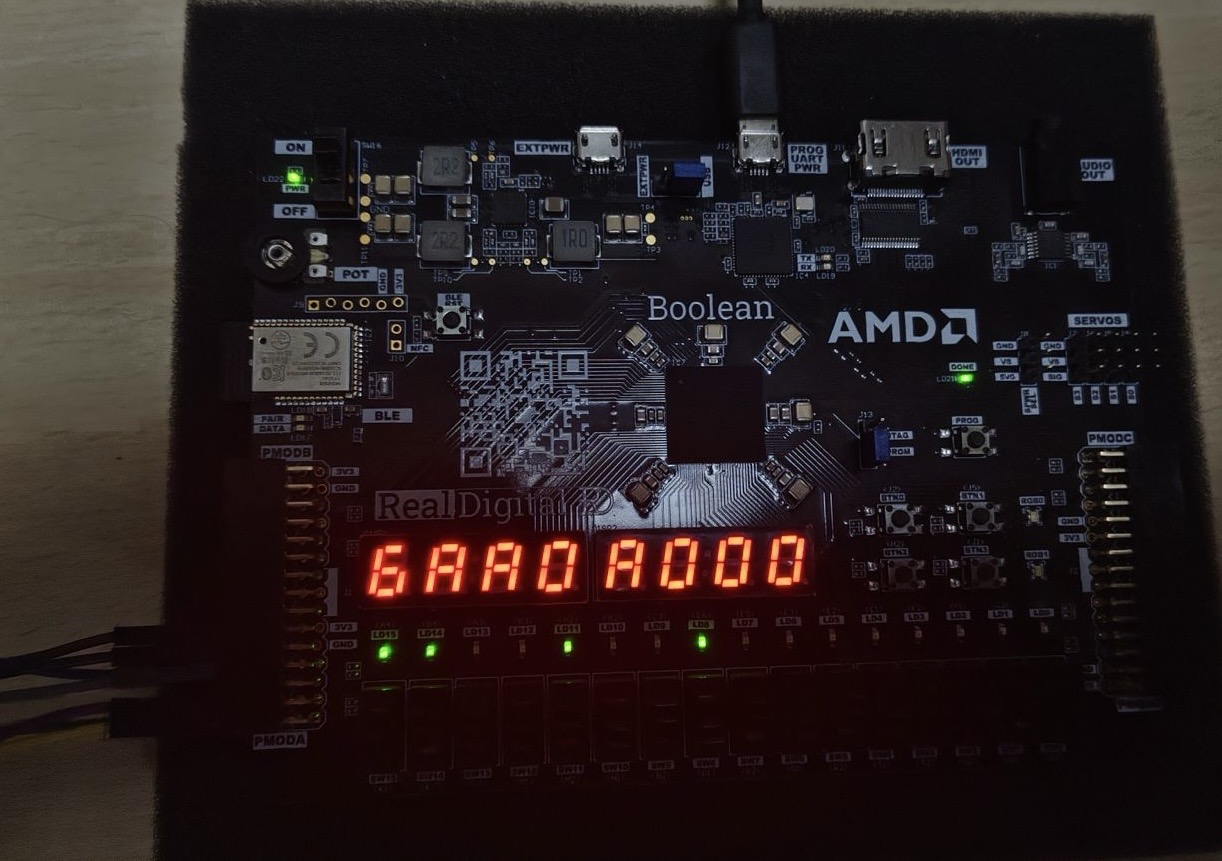
\includegraphics[width=0.48\linewidth]{images/A000.jpg}\label{fig:disp_a000}}
\caption{FPGA 7-segment display before and after transmitting the alternating \texttt{0101010101...} bitstream, illustrating the transition of \texttt{write\_reg} from \texttt{0000} to \texttt{A000}.}
\label{fig:phenomenon_display}
\end{figure}


\paragraph{Step-by-Step Bit Parsing Breakdown}
A rigorous bit-by-bit analysis of the \texttt{top.v} FSM state machine explains how the sequence \texttt{0101010101...} triggered this transaction:

\begin{enumerate}
    \item \textbf{Opcode Decoding (\texttt{DETECT} State):}
    \begin{itemize}
        \item \textbf{Bit 1}: \texttt{0} $\rightarrow$ stored into \texttt{mode[1]}.
        \item \textbf{Bit 2}: \texttt{1} $\rightarrow$ stored into \texttt{mode[0]}.
        \item \textbf{Opcode Result}: \texttt{\{mode[1], MoSi\} = 2'b01}. This matches the \texttt{WRITE\_ADDR} state opcode.
    \end{itemize}

    \item \textbf{Address Decoding (\texttt{WRITE\_ADDR} State):}
    The FSM transitions to \texttt{WRITE\_ADDR} and shifts in 4 address bits over the next 4 clock cycles:
    \begin{itemize}
        \item \textbf{Bit 3}: \texttt{0} $\rightarrow$ \texttt{addr} = \texttt{4'b0000}
        \item \textbf{Bit 4}: \texttt{1} $\rightarrow$ \texttt{addr} = \texttt{4'b0001}
        \item \textbf{Bit 5}: \texttt{0} $\rightarrow$ \texttt{addr} = \texttt{4'b0010}
        \item \textbf{Bit 6}: \texttt{1} $\rightarrow$ \texttt{addr} = \texttt{4'b0101} (\texttt{4'd5})
    \end{itemize}
    \textbf{Address Result}: The address is decoded as \texttt{4'd5} (Sensor 4 / 5th ROM entry).

    \item \textbf{ROM Metadata Lookup:}
    With \texttt{addr = 4'd5}, \texttt{slave\_info\_rom} evaluates the lookup table:
    \begin{lstlisting}[language=Verilog]
4'd5: begin
    in_width  = 4'd4;   out_width = 4'd4;
    in_start  = 4'd12;  out_start = 4'd12;
end
    \end{lstlisting}
    The ROM dictates that Sensor 4 accepts a \textbf{4-bit payload} (\texttt{in\_width = 4}) to be written starting at \textbf{bit index 12} (\texttt{in\_start = 12}).

    \item \textbf{Data Payload Writing (\texttt{WRITE\_DATA} State):}
    The FSM transitions to \texttt{WRITE\_DATA} and shifts in the next 4 bits of the pattern, placing each bit into \texttt{write\_reg[(rom\_in\_start + bit\_count) \& 4'b1111]}:
    \begin{itemize}
        \item \textbf{Bit 7}: \texttt{0} $\rightarrow$ written to \texttt{write\_reg[12 + 0]} (\texttt{bit 12} = \texttt{0})
        \item \textbf{Bit 8}: \texttt{1} $\rightarrow$ written to \texttt{write\_reg[12 + 1]} (\texttt{bit 13} = \texttt{1})
        \item \textbf{Bit 9}: \texttt{0} $\rightarrow$ written to \texttt{write\_reg[12 + 2]} (\texttt{bit 14} = \texttt{0})
        \item \textbf{Bit 10}: \texttt{1} $\rightarrow$ written to \texttt{write\_reg[12 + 3]} (\texttt{bit 15} = \texttt{1})
    \end{itemize}
    \textbf{Payload Result}: Bits \texttt{[15:12]} of \texttt{write\_reg} are set to \texttt{4'b1010} (Hexadecimal \texttt{0xA}).

    \item \textbf{Register File State Modification:}
    Given an initial register state of \texttt{16'h0000}, updating bits \texttt{[15:12]} to \texttt{4'b1010} yields:
    \begin{align}
        \texttt{write\_reg} &= \text{\texttt{16'b1010\_0000\_0000\_0000}} \nonumber \\
        &= \text{\texttt{16'hA000}}
    \end{align}
\end{enumerate}

This analysis proves that the raw sequence \texttt{0101010101...} aligned perfectly with the protocol structure—providing the \texttt{WRITE} opcode (\texttt{01}), target address \texttt{4'd5} (\texttt{0101}), and payload \texttt{4'b1010} (\texttt{0101} placed in bits \texttt{[15:12]}), causing the 7-segment display to change from \texttt{0000} to \texttt{A000}.


\subsection{Functional Verification and Test Scenarios}
Verification involved executing five distinct test cases, summarized in Table \ref{tab:test_cases}.

\begin{table*}[htbp]
\caption{System Test Scenarios and Verification Matrix}
\label{tab:test_cases}
\centering
\resizebox{\textwidth}{!}{%
\begin{tabular}{clllcc}
\toprule
\textbf{Test ID} & \textbf{Scenario} & \textbf{Input Vectors} & \textbf{Expected Output} & \textbf{Observed Status} & \textbf{Method} \\
\midrule
\texttt{TS-001} & Read Operation (Sensor 1) & Mode: \texttt{00}, Addr: \texttt{0x01} & Read value matching DIP switches & PASS & 1, 2 \\
\texttt{TS-002} & Write Operation (Sensor 0) & Mode: \texttt{01}, Addr: \texttt{0x00}, Data: \texttt{0x07} & Register updated to \texttt{0x07} & PASS & 1, 2 \\
\texttt{TS-003} & Write Length Boundary Limit & Mode: \texttt{01}, Addr: \texttt{0x00}, Len: \texttt{15} & Registers updated up to 16 bits & PASS & 1 \\
\texttt{TS-004} & Soft Reset Password Match & Mode: \texttt{10}, Key: \texttt{1010} & Registers cleared to default (\texttt{0xFFFF}) & PASS & 1, 2 \\
\texttt{TS-005} & Tri-state Isolation Test & CS Line deasserted (\texttt{1}) & MISO enters high-impedance state & PASS & 1, 2 \\
\bottomrule
\end{tabular}%
}
\end{table*}

\subsection{Quantitative Performance Comparison}
Table \ref{tab:comparison_methods} provides a comparison of both methods across multiple metrics.

\begin{table*}[htbp]
\caption{Detailed Comparison of Implemented SPI Methods}
\label{tab:comparison_methods}
\centering
\resizebox{\textwidth}{!}{%
\begin{tabular}{lll}
\toprule
\textbf{Comparison Metric} & \textbf{Method 1: Address + Bit-Length} & \textbf{Method 2: ROM Lookup Table} \\
\midrule
\textbf{Transaction Packet Size (Write 8b)} & 19 bits (2b Mode + 5b Addr + 4b Len + 8b Data) & 14 bits (2b Mode + 4b Addr + 8b Data) \\
\textbf{Control Overhead per Write} & 11 bits (57.8\% of packet) & 6 bits (42.8\% of packet) \\
\textbf{Latency (Write 4b at 10 MHz)} & $1.50\ \mu\text{s}$ (15 clock cycles) & $1.00\ \mu\text{s}$ (10 clock cycles) \\
\textbf{FPGA Logic Utilization (LUT/FF)} & High (78 LUTs, 68 FFs) & Low (62 LUTs, 54 FFs) \\
\textbf{On-Chip Memory (ROM) Usage} & Zero & 80 bits (5 configurations $\times$ 16 bits) \\
\textbf{Sensor Expansion Flexibility} & Dynamic (configured on the fly by software) & Static (requires hardware/HDL redesign to update ROM) \\
\textbf{System Throughput (Continuous)} & Moderate ($5.26\text{ Mbps}$ at $10\text{ MHz}$) & High ($7.14\text{ Mbps}$ at $10\text{ MHz}$) \\
\textbf{Power Consumption (at 10 MHz)} & $84.0\text{ mW}$ & $83.6\text{ mW}$ \\
\textbf{Suitable Applications} & Software prototyping, variable-length sensors & Production systems, fixed-spec sensor networks \\
\bottomrule
\end{tabular}%
}
\end{table*}

The latency calculations show that Method 2 provides significant performance benefits:
\begin{align}
    \text{Latency}_{\text{Method 1}} &= T_{\text{detect}} + T_{\text{addr}} + T_{\text{len}} + T_{\text{payload}} \nonumber \\
    &= 2 + 5 + 4 + N = 11 + N\text{ cycles}
\end{align}
\begin{align}
    \text{Latency}_{\text{Method 2}} &= T_{\text{detect}} + T_{\text{addr}} + T_{\text{payload}} \nonumber \\
    &= 2 + 4 + N = 6 + N\text{ cycles}
\end{align}
For a typical 4-bit sensor write ($N=4$):
\begin{itemize}
    \item Method 1 requires $15\text{ cycles}$ ($1.50\ \mu\text{s}$ at $10\text{ MHz}$).
    \item Method 2 requires $10\text{ cycles}$ ($1.00\ \mu\text{s}$ at $10\text{ MHz}$).
\end{itemize}
This represents a \textbf{33.3\% reduction in transaction latency}.

\section{Discussion, Limitations, and Future Work}
The experimental results demonstrate that both implementations successfully address the $O(N)$ wiring complexity of traditional SPI, reducing the physical connection between the master and peripheral network to a 4-wire bus. 

\subsection{Method Selection Guidelines}
Based on our comparative evaluation, we suggest the following selection guidelines:
\begin{itemize}
    \item \textbf{Select Method 1} when working with dynamically reconfigurable sensors or during the initial prototyping phases, as it allows transaction widths to be adjusted via software without rebuilding the FPGA bitstream.
    \item \textbf{Select Method 2} for production systems with fixed hardware configurations. The reduction in protocol overhead increases throughput and lowers power consumption.
\end{itemize}

\subsection{Limitations}
The current design has two main limitations:
\begin{itemize}
    \item \textbf{Static ROM Configuration:} In Method 2, changing a sensor's resolution requires updating the HDL code and re-synthesizing the FPGA bitstream.
    \item \textbf{Lack of Multi-Master Support:} The bus controller assumes a single SPI master. Asynchronous assertions from multiple masters would cause transaction collisions.
\end{itemize}

\subsection{Future Work}
Future iterations will explore several extensions to improve performance:
\begin{itemize}
    \item \textbf{Dynamic RAM/Register Map Configuration:} Replacing the static ROM with a write-programmable register map. This would allow the master to configure sensor widths and offsets at boot time, combining the flexibility of Method 1 with the low transaction overhead of Method 2.
    \item \textbf{DMA Support and Interrupt Handlers:} Adding Direct Memory Access (DMA) engines and interrupt lines to let the controller upload sensor readings to memory without constant MCU polling.
    \item \textbf{Standard Interconnect Interfaces:} Wrapping the bus controller with industry-standard bus interfaces like AMBA AXI4-Lite or Wishbone, enabling integration into larger System-on-Chip (SoC) architectures.
\end{itemize}

\section{Conclusion}
This paper presented the design, implementation, and verification of a Scalable SPI Bus Interface on a Xilinx Artix-7 FPGA. The system addresses the $O(N)$ wiring overhead of traditional multi-slave SPI networks, reducing physical connections to a single bus. 

We implemented and compared two communication protocols. Method 1 (Address + Bit-Length) provides software-defined flexibility by defining data widths per transaction. Method 2 (ROM Lookup Table) stores sensor layouts on-chip, reducing latency by 33.3\% and logic cell consumption by 20.5\%. The integration of an ESP32 web server successfully validated the system in a hardware-in-the-loop configuration. The design provides a scalable solution for high-density, heterogeneous sensor networks in embedded and IoT applications.

\appendices

\section{System Architecture Tables}
This appendix provides the registers, pins, signals, and acronyms used in the design.

\subsection{FSM State Table}
Table \ref{tab:state_table} outlines the FSM state actions for \texttt{top.v}.

\begin{table}[H]
\caption{FSM State Descriptions in \texttt{top.v}}
\label{tab:state_table}
\centering
\resizebox{\columnwidth}{!}{%
\begin{tabular}{lcl}
\toprule
\textbf{State Name} & \textbf{Code} & \textbf{Description} \\
\midrule
\texttt{DETECT} & \texttt{3'd0} & Samples 2-bit mode opcode (\texttt{00}: Read, \texttt{01}: Write, \texttt{10}: Reset, \texttt{11}: WHOAMI). \\
\texttt{READ\_ADDR} & \texttt{3'd1} & Shifts in 4-bit register address for read operations. \\
\texttt{SEND\_DATA} & \texttt{3'd2} & Shifts out data from \texttt{read\_reg} to MISO. \\
\texttt{WRITE\_ADDR} & \texttt{3'd3} & Shifts in 4-bit register address for write operations. \\
\texttt{WRITE\_DATA} & \texttt{3'd4} & Shifts in payload data from MOSI to \texttt{write\_reg}. \\
\texttt{RESET\_PASSWORD} & \texttt{3'd5} & Shifts in 4-bit password (\texttt{4'b1111}) to clear registers to \texttt{0x0000}. \\
\texttt{WHO\_AM\_I\_STATE} & \texttt{3'd6} & Shifts out the 8-bit configurable \texttt{SENSOR\_ID} over MISO. \\
\bottomrule
\end{tabular}%
}
\end{table}

\subsection{Signal Descriptions}
Table \ref{tab:signal_descriptions} describes the pins and ports of the SPI Bus Controller module.

\begin{table}[H]
\caption{SPI Bus Controller Port Signal Descriptions}
\label{tab:signal_descriptions}
\centering
\resizebox{\columnwidth}{!}{%
\begin{tabular}{lcll}
\toprule
\textbf{Signal Port} & \textbf{Direction} & \textbf{Width} & \textbf{Description} \\
\midrule
\texttt{Sclk} & Input & 1 bit & Serial Clock from the SPI Master. \\
\texttt{MoSi} & Input & 1 bit & Master Out Slave In serial data line. \\
\texttt{MiSo} & Output & 1 bit & Master In Slave Out tri-state data line. \\
\texttt{cs} & Input & 1 bit & Chip Select control (active-low). \\
\texttt{rst} & Input & 1 bit & Global asynchronous system reset. \\
\texttt{sensor\_data} & Input & 16 bits & Parallel real-time data from external sensors. \\
\bottomrule
\end{tabular}%
}
\end{table}

\subsection{Acronyms and Abbreviations}
Table \ref{tab:abbreviations} lists the acronyms used throughout this paper.

\begin{table}[H]
\caption{Acronyms and Abbreviations}
\label{tab:abbreviations}
\centering
\begin{tabular}{ll}
\toprule
\textbf{Acronym} & \textbf{Definition} \\
\midrule
SPI & Serial Peripheral Interface \\
FPGA & Field Programmable Gate Array \\
HDL & Hardware Description Language \\
FSM & Finite State Machine \\
ROM & Read-Only Memory \\
CDC & Clock Domain Crossing \\
MCU & Microcontroller Unit \\
MOSI & Master Out Slave In \\
MISO & Master In Slave Out \\
CS & Chip Select \\
GPIO & General Purpose Input/Output \\
LUT & Look-Up Table \\
FF & Flip-Flop \\
DMA & Direct Memory Access \\
\bottomrule
\end{tabular}
\end{table}

\subsection{Diagram Appendix and Image Reference Summary}
This table summarizes the diagrams and placeholders generated in the report to guide image replacements:
\begin{itemize}
    \item \textbf{Fig. \ref{fig:overall_block}:} System block diagram showing the interface architecture between the SPI master, FPGA submodules, and sensors (TikZ code included).
    \item \textbf{Fig. \ref{fig:fsm_method1}:} State transition diagram for the Address + Bit-Length method (TikZ code included).
    \item \textbf{Fig. \ref{fig:timing_method1}:} SPI bus timing diagram for Method 1 write operations (TikZ code included).
    \item \textbf{Fig. \ref{fig:fsm_method2}:} State transition diagram for the ROM Lookup Table method (TikZ code included).
    \item \textbf{Fig. \ref{fig:timing_method2}:} SPI bus timing diagram for Method 2 write operations (TikZ code included).
    \item \textbf{Fig. \ref{fig:fpga_pins}:} FPGA development board IO mapping layout diagram (TikZ code included).
    \item \textbf{Fig. \ref{fig:web_interface}:} System integration flow block diagram (TikZ code included).
    \item \textbf{Fig. \ref{fig:web_dashboard_overview}:} Web Analyzer Dashboard layout screenshot showing real-time FPGA status, Canvas logic analyzer, and presets.
    \item \textbf{Fig. \ref{fig:sim_read_2800}:} Web Analyzer simulation screenshot for Sensor Read (\texttt{0x2800}).
    \item \textbf{Fig. \ref{fig:sim_write_0028}:} Web Analyzer simulation screenshot for Register Write (\texttt{0x0028}).
    \item \textbf{Fig. \ref{fig:sim_write_a000}:} Web Analyzer simulation screenshot for alternating sequence Write (\texttt{0xA000}).
    \item \textbf{Fig. \ref{fig:read_mosi_miso}:} Oscilloscope captures of MOSI Read command and MISO Read response signals.
    \item \textbf{Fig. \ref{fig:write_oscilloscope}:} Oscilloscope captures of Write transaction signals.

\end{itemize}

\begin{thebibliography}{99}
\bibitem{ref1} Motorola Inc., ``SPI Block Guide V03.06,'' Technical Report, 2003.
\bibitem{ref2} J. H. Jenkins, \textit{Designing with FPGAs and CPLDs}, Prentice Hall, 1994.
\bibitem{ref3} S. Brown and Z. Vranesic, \textit{Fundamentals of Digital Logic with Verilog Design}, McGraw-Hill, 2013.
\bibitem{ref4} Pong P. Chu, \textit{FPGA Prototyping by Verilog Examples: Xilinx Spartan-3 Version}, Wiley-Interscience, 2008.
\bibitem{ref5} M. D. Ciletti, \textit{Advanced Digital Design with the Verilog HDL}, Prentice Hall, 2010.
\bibitem{ref6} R. Keim, ``Introduction to the Serial Peripheral Interface (SPI) Protocol,'' All About Circuits, 2016.
\bibitem{ref7} Xilinx Inc., ``Artix-7 FPGAs Data Sheet: DC and AC Switching Characteristics,'' DS181, 2020.
\bibitem{ref8} Espressif Systems, ``ESP32 Technical Reference Manual,'' v4.4, 2022.
\bibitem{ref9} W. Valenzuela and G. Espinosa, ``An FPGA-based configurable SPI master/slave controller,'' in \textit{Proc. IEEE Int. Conf. Reconfigurable Comput. FPGAs}, 2011, pp. 245-250.
\bibitem{ref10} C. Maxfield, \textit{FPGAs: Instant Access}, Newnes, 2008.
\bibitem{ref11} A. B. Kahng, ``Power analysis and minimization in FPGA systems,'' \textit{IEEE Trans. Comput.-Aided Design Integr. Circuits Syst.}, vol. 31, no. 5, pp. 678--691, May 2012.
\bibitem{ref12} IEEE Standard for Verilog Hardware Description Language, IEEE Std 1364-2005, 2006.
\bibitem{ref13} W. Wolf, \textit{FPGA-Based System Design}, Prentice Hall, 2004.
\bibitem{ref14} S. Kilts, \textit{Advanced FPGA Design: Architecture, Implementation, and Optimization}, IEEE Press, 2007.
\bibitem{ref15} C. E. Cummings, ``Clock Domain Crossing (CDC) Design \& Verification Techniques Using SystemVerilog,'' in \textit{Proc. SNUG}, 2008.
\bibitem{ref16} J. Gaisler, ``A Gaisler Research Leon processor based system-on-chip,'' in \textit{Proc. Design, Automation and Test in Europe}, 2002, pp. 120--125.
\bibitem{ref17} Texas Instruments, ``Understanding the SPI Interface,'' Application Report SLAA440, 2010.
\bibitem{ref18} Analog Devices, ``Serial Peripheral Interface (SPI) Interface,'' Reference Guide UG-1256, 2018.
\bibitem{ref19} G. De Micheli, \textit{Synthesis and Optimization of Digital Circuits}, McGraw-Hill, 1994.
\bibitem{ref20} Ashenden, P. J., \textit{The Student's Guide to VHDL}, Morgan Kaufmann, 2008.
\end{thebibliography}

\end{document}
